% !TEX TS-program = pdflatex
% !TEX encoding = UTF-8 Unicode

% This is a simple template for a LaTeX document using the "article" class.
% See "book", "report", "letter" for other types of document.

\documentclass[11pt,abstracton]{scrreprt} % use larger type; default would be 10pt

\usepackage[utf8]{inputenc} % set input encoding (not needed with XeLaTeX)
\usepackage{german}
%%% Examples of Article customizations
% These packages are optional, depending whether you want the features they provide.
% See the LaTeX Companion or other references for full information.

%%% PAGE DIMENSIONS
\usepackage{geometry} % to change the page dimensions
\geometry{a4paper} % or letterpaper (US) or a5paper or....
% \geometry{margins=2in} % for example, change the margins to 2 inches all round
% \geometry{landscape} % set up the page for landscape
%   read geometry.pdf for detailed page layout information

\usepackage{graphicx} % support the \includegraphics command and options

% \usepackage[parfill]{parskip} % Activate to begin paragraphs with an empty line rather than an indent

%%% PACKAGES
\usepackage{booktabs} % for much better looking tables
\usepackage{array} % for better arrays (eg matrices) in maths
\usepackage{paralist} % very flexible & customisable lists (eg. enumerate/itemize, etc.)
\usepackage{verbatim} % adds environment for commenting out blocks of text & for better verbatim
\usepackage{subfig} % make it possible to include more than one captioned figure/table in a single float
\usepackage{german}
\usepackage{url}
\usepackage[colorlinks=true]{hyperref}
\usepackage{amsfonts}
\usepackage{amsmath}
\usepackage{amsthm}
\usepackage{listings}
\usepackage{tikz}
\usepackage{pgfplots}
\usetikzlibrary{arrows,%
                petri,%
                topaths}%
\usepackage{tkz-berge}
\usepackage{algorithm}% http://ctan.org/pkg/algorithms
\usepackage{algpseudocode}% http://ctan.org/pkg/algorithmicx
% These packages are all incorporated in the memoir class to one degree or another...

\usepackage{listings}
\usepackage{color}
\definecolor{lightgray}{rgb}{.9,.9,.9}
\definecolor{darkgray}{rgb}{.4,.4,.4}
\definecolor{purple}{rgb}{0.65, 0.12, 0.82}

\lstdefinelanguage{JavaScript}{
  keywords={typeof, new, true, false, catch, function, return, null, catch, switch, var, if, in, while, do, else, case, break},
  keywordstyle=\color{blue}\bfseries,
  ndkeywords={class, export, boolean, throw, implements, import, this},
  ndkeywordstyle=\color{darkgray}\bfseries,
  identifierstyle=\color{black},
  sensitive=false,
  comment=[l]{//},
  morecomment=[s]{/*}{*/},
  commentstyle=\color{purple}\ttfamily,
  stringstyle=\color{red}\ttfamily,
  morestring=[b]',
  morestring=[b]"
}

\lstset{
   language=JavaScript,
   backgroundcolor=\color{lightgray},
   extendedchars=true,
   basicstyle=\footnotesize\ttfamily,
   showstringspaces=false,
   showspaces=false,
   %numbers=left,
   numberstyle=\footnotesize,
   numbersep=9pt,
   tabsize=2,
   breaklines=true,
   showtabs=false,
   captionpos=b
}

%%% HEADERS & FOOTERS
\usepackage{fancyhdr} % This should be set AFTER setting up the page geometry
\pagestyle{fancy} % options: empty , plain , fancy
\renewcommand{\headrulewidth}{0pt} % customise the layout...
\lhead{}\chead{}\rhead{}
\lfoot{}\cfoot{\thepage}\rfoot{}

%%% SECTION TITLE APPEARANCE
\usepackage{sectsty}
\allsectionsfont{\sffamily\mdseries\upshape} % (See the fntguide.pdf for font help)
% (This matches ConTeXt defaults)

%%% ToC (table of contents) APPEARANCE
\usepackage[nottoc,notlof,notlot]{tocbibind} % Put the bibliography in the ToC
\usepackage[titles,subfigure]{tocloft} % Alter the style of the Table of Contents
\renewcommand{\cftsecfont}{\rmfamily\mdseries\upshape}
\renewcommand{\cftsecpagefont}{\rmfamily\mdseries\upshape} % No bold!

%%% END Article customizations

%%% The "real" document content comes below...

\theoremstyle{definition}
\newtheorem*{beisp}{Beispiel}
\newtheorem{definition}{Definition}
\newtheorem*{bemerkung}{Bemerkung}

\title{Graph Coloring als Online-Problem mit bipartiten Graphen und Advice Complexity}
\subtitle{Semesterarbeit}
\author{Florian Lüthi\footnote{\url{luethifl@students.zhaw.ch}}}
\date{ZHAW, 22. Dezember 2013} % Activate to display a given date or no date (if empty),
         % otherwise the current date is printed 

\begin{document}
\maketitle

\begin{abstract}
Diese Semesterarbeit beschäftigt sich mit dem Verhältnis zwischen Online- und Offline-Problemen. Ausserdem gibt sie einen Überblick über das Konzept der {\sl Advice Complexity} sowie deren Anwendung zur Erreichung einer konstanten Competitive Ratio für einen Graphenfärbe-Algorithmus auf bipartiten Zufallsgraphen. Die dazu notwendigen Modelle werden ebenfalls erläutert. Sie verifiziert empirisch die theoretische obere Schranke an Advice Bits von $b = \frac n {\sqrt{ 2 ^ {k-1 }}}$ (\cite{bipartite}) und erläutert das dazu notwendige Programm. Schlussendlich führt sie einige Experimente durch, um einen allfälligen Zusammenhang zwischen der Länge und der Kantendichte von bipartiten Zufallsgraphen sowie der Competitive Ratio und der Menge an Advice Bits des entsprechenden Online-Algorithmus zu finden. Sie vermutet, dass die Kantendichte als Teil der Länge aufgefasst werden sollte.
\end{abstract}

\tableofcontents

\chapter{Einleitung}

Selbst in Zeiten immer grösser werdender Datenmengen, stetig wachsender verfügbarer Rechenleistung sowie daraus folgender immens gestiegener Erwartungen an die digitalisierte und automatisierte Welt bleibt die (aus menschlicher Sicht beruhigende) Erkenntnis, dass selbst die unmittelbare Zukunft unerwartete Wendungen beinhaltet.

\bigskip

Diese Arbeit beschäftigt sich in dem ihr vorgegebenen Rahmen zur Hauptsache mit den beiden Konzepten Advice Complexity und Graphenfärbung. Zusammen mit dem Programm {\tt GraphBonanza}\footnote{\url{https://github.com/foyan/GraphBonanza}} versucht sie einen Überblick über diese Themen zu geben, sowie ein Theorem aus \cite{bipartite} experimentell zu verifizieren.

Diese Arbeit ist folgendermassen aufgebaut: Im nächsten Kapitel wird auf das Konzept der Advice Complexity eingegangen, im Übernächsten auf dasjenige der Graphenfärbung, in Kapitel 4 werden diese beiden Themen miteinander verknüpft und es werden Experimente durchgeführt. Im letzten Kapitel folgt eine kurze Kommentierung der Implementation von {\tt GraphBonanza}.

\bigskip
Der Autor bedankt sich bei Dr. Lucia Keller für die sehr kompetente Betreuung sowie die terminliche Flexibilität. Derselbe Dank gilt auch der Studienleitung.


\chapter{Advice Complexity}

\section{Online- vs. Offline-Probleme}

Optimierungsprobleme lassen sich (unter vielerlei anderen Klassifikationsmöglichkeiten) in Online-Probleme und Offline-Probleme mit dazugehörigen Online- bzw. Offline-Algo\-rithmen unterteilen. Der wesentliche Unterschied zwischen diesen beiden Klassen besteht darin, dass ein Offline-Algorithmus seine gesamte Eingabe zur Laufzeit kennt, während ein Online-Algorithmus dies nicht tut. Er bekommt einen Teil der Eingabe und berechnet daraus sofort einen Teil des Resultats. Ein solches Teilresultat kann im Nachhinein nicht mehr geändert werden.

Es liegt nun auf der Hand, dass ein Online-Algorithmus dazu tendiert, während der Berechnung eines Teilresultats Entscheidungen zu treffen, welche sich nach Berechnungen weiterer Teilresultate als suboptimal herausstellen -- dies insbesondere darum, weil die während der Berechnung des Teilresultats $i$ zur Verfügung stehenden Informationen über das gesamte Problem nur aus den Teileingaben der Berechnungen $1$ bis $i$ stammen können \cite{BKK}.

\bigskip
Eine weitere Folge des obengenannten Unterschieds manifestiert sich darin, dass ein Offline-Algorithmus prinzipiell immer eine optimale Lösung finden kann, während der entsprechende Online-Algorithmus unter Umständen zu wenig Informationen zur Verfü\-gung hat. Dies verunmöglicht den Vergleich dieser beiden Typen von Algorithmen mittels klassischer Masse wie zum Beispiel der asymptotischen Laufzeitkomplexität. Aus diesem Grunde muss eine andere Möglichkeit gefunden werden, einen Offline-Algorithmus mit seinem Online-Pendant (und deren Lösungen) vergleichen zu können.

\section{Competitive Ratio}

Eine gängige Möglichkeit dafür ist die von Sleator und Tarjan eingeführte {\it Competitive Ratio} \cite{Sleator, BKK}, welche im Grunde genommen das Verhältnis zwischen den Kosten der optimalen Lösung und derer des zu untersuchenden Online-Algorithmus ausdrückt \cite{BKK}. Da die Qualität der Lösung eines Online-Algorithmus wesentlich von der Beschaffenheit der Eingabe abhängt, wird dabei vom jeweils schlechtestmöglichen Fall ausgegangen \cite{Trevisan}.

\bigskip
Formal kann die Competitive Ratio folgendermassen definiert werden: Sei $\operatorname{opt}(I)$ die optimale Lösung eines konkreten Online-Problems für eine Sequenz aus Teileingaben $I$, welche durch einen Offline-Algorithmus erreicht werden kann.
% $\mathcal{I}$ sei die Menge aller möglicher solcher Sequenzen.
Seien ferner $\mathcal{S}$ alle möglichen Lösungen (mit $\operatorname{opt}(I) \in \mathcal{S}$), $A(I) \in \mathcal{S}$ diejenige Lösung, welche der Online-Algorithmus $A$ zu diesem Problem liefern kann, und $C : \mathcal{S} \rightarrow \mathbb{R}$ die Kosten für die jeweilige Lösung.

\bigskip
Ein Online-Algorithmus $A$ für ein Minimierungsproblem wird nun als {\it $c$-kompetitiv} bezeichnet, wenn es Konstanten $c \ge 0$ und $\alpha$ gibt, sodass für sämtliche mögliche Eingaben $I$
\[
C(A(I)) \le c\cdot C(\operatorname{opt}(I)) + \alpha
\]
gilt \cite{BKK}.
% und die Competitive Ratio wäre ergo
%\[
%c = \max_{I \in \mathcal{I}} \left\{ \frac {C(A(I))}{C(\operatorname{opt}(I))} \right\}.
%\]

Ausserdem bezeichnen wir einen Algorithmus $A$ von nun an als {\sl kompetitiv}, wenn es ein solches $c$ gibt (sprich wenn die Competitive Ratio nicht von der Eingabelänge $n$ abhängt).

\section{Das {\sc SkiRental}-Problem}

Die Competitive Ratio lässt sich durch das wohlbekannte {\sc SkiRental}-Problem illustrieren: Nehmen wir an, wir wollen zum ersten Mal ein Wochenende lang Skifahren gehen. Wir besitzen aber keine Skis. Es stellt sich nun die Frage, ob wir Skis mieten oder kaufen wollen -- wobei erschwerend hinzukommt, dass wir momentan noch keine Ahnung haben, wieviele Wochenenden wir danach noch skifahrend verbringen möchten.

Angenommen, der Kauf eines Paars Ski kostet CHF 500, die Miete äquivalenter Skis für ein Wochenende hingegen CHF 50.\footnote{In der Realität wesentliche Aspekte wie Preisveränderungen über die Zeit, veränderte Qualitätsansprüche und Abnützung der Skis sollen bei dieser Betrachtung vernachlässigt werden.} Es ist nun einfach auszurechnen, dass sich der Kauf der Skis vor dem ersten Wochenende nur lohnen würde, wenn wir an mindestens 10 Wochenenden Skifahren gehen würden.

\bigskip
Da wir das aber nicht wissen, sind wir gezwungen, von Anfang an einen Online-Algorithmus $A_t$ auszuwählen, der für jede Teileingabe (sprich für jedes geplante Skiwochenende) sofort die Frage nach Kauf oder Miete beantworten muss. Die Teileingabe für den Algorithmus ist jeweils die Anzahl an vergangenen Skiwochenenden.

Die oben besprochene Eigenschaft der potenziellen Suboptimalität der Entscheidungen wird beim zehnten solchen Wochenende augenscheinlich, wenn bei den vorangegangen Wochenenden die Entscheidung jeweils auf Mieten gefallen sein sollte.

\bigskip
Bezeichne $t$ nun dasjenige Wochenende, an welchem wir uns dafür entscheiden, die Skis zu kaufen. Wir schauen uns die folgenden Fälle an:

\begin{itemize}
\item Für $t = 1$ gilt, dass $A_1(I) = 500$, denn wir kaufen ja gleich beim ersten Mal. Die Competitive Ratio $c$ hingegen liegt bei $10$, da wir im schlechtesten Fall nur dieses eine Mal Skifahren gehen -- es gälte also $\operatorname{opt}_1(I) = 50$.

\item Für $t = 2$ gilt, dass $A_2(I) = 550$, denn wir mieten beim ersten (CHF 50) und kaufen beim zweiten Mal (CHF 500). Die Competitive Ratio $c$ liegt bei $5.5$, da wir im schlechtesten Fall nur diese zwei Male Skifahren gehen -- optimal wäre zwei Mal mieten, also  $\operatorname{opt}_2(I) = 100$.

\item Für $t = 10$ gilt, dass $A_{10}(I) = 950$, denn wir mieten die ersten neun Male (CHF 450) und kaufen beim zehnten Mal (CHF 500). Für die optimale Lösung spielt es keine Rolle, ob jeweils gemietet oder von Anfang an gekauft wird, also ist $\operatorname{opt}_{10}(I) = 500$. Dies ergibt eine Competitive Ratio von $c = 1.9$.

\item Für $t = 11$ gilt, dass $A_{11}(I) = 1000$, denn wir mieten die ersten zehn Male (CHF 500) und kaufen beim elften Mal (CHF 500). Die Competitive Ratio $c$ liegt bei $c = 2$, da es optimal wäre, gleich beim ersten Mal die Skis zu kaufen (CHF 500).
\end{itemize}

Der Verlauf von $\operatorname{opt}_t(I)$ und $A_t(I)$ in Abhängigkeit von $t$ ist in Abbildung \ref{fig.skirental} skizziert, Abbildung \ref{fig.skirental.c} zeigt $c$ in Abhängigkeit von $t$.

\begin{figure}
\caption{Verlauf von Lösung und Optimum für SkiRental}
\label{fig.skirental}
\begin{center}
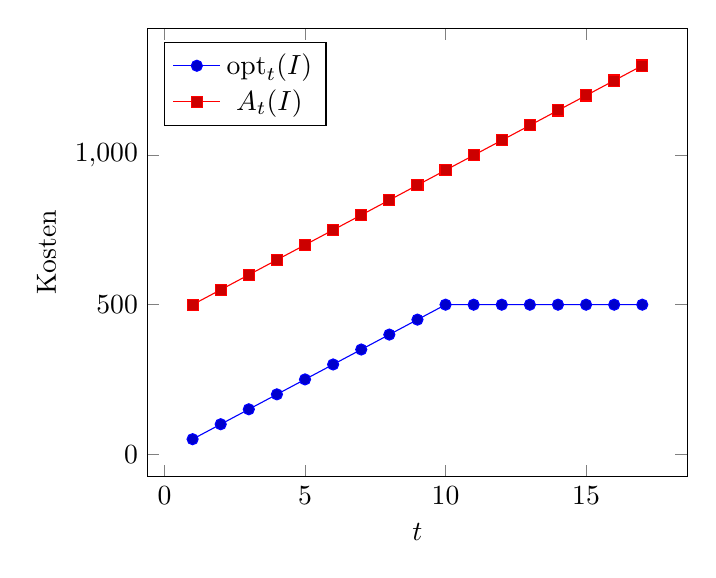
\begin{tikzpicture}
  \begin{axis}[ 
    xlabel=$t$,
    ylabel={Kosten},
	legend pos=north west
  ] 
    \addplot coordinates {
		(1,50)
		(2,100)
		(3,150)
		(4,200)
		(5,250)
		(6,300)
		(7,350)
		(8,400)
		(9,450)
		(10,500)
		(11,500)
		(12,500)
		(13,500)
		(14,500)
		(15,500)
		(16,500)
		(17,500)
	};
	\addlegendentry{$\operatorname{opt}_t(I)$}
    \addplot coordinates {
		(1,500)
		(2,550)
		(3,600)
		(4,650)
		(5,700)
		(6,750)
		(7,800)
		(8,850)
		(9,900)
		(10,950)
		(11,1000)
		(12,1050)
		(13,1100)
		(14,1150)
		(15,1200)
		(16,1250)
		(17,1300)
	};
	\addlegendentry{$A_t(I)$}
  \end{axis}
\end{tikzpicture}
\end{center}
\end{figure}

\begin{figure}
\caption{Verlauf der Competitive Ratio für SkiRental}
\label{fig.skirental.c}
\begin{center}
\begin{tikzpicture}
  \begin{axis}[ 
    xlabel=$t$,
    ylabel={$c(t)$},
	legend pos=north west
  ] 
    \addplot coordinates {
		(1,10)
		(2,5.5)
		(3,4)
		(4,3.25)
		(5,2.8)
		(6,2.5)
		(7,2.2857142857)
		(8,2.125)
		(9,2)
		(10,1.9)
		(11,2)
		(12,2.1)
		(13,2.2)
		(14,2.3)
		(15,2.4)
		(16,2.5)
		(17,2.6)
	};
  \end{axis}
\end{tikzpicture}
\end{center}
\end{figure}

\bigskip
Allgemein kann die Competitive Ratio für dieses Problem (mit allgemeinen Kosten $b$ für den Kauf bzw. $r$ für die Miete) beschrieben werden als
\[
	c(t) = \begin{cases}
		\frac{b+(t-1)\cdot r}{t\cdot r}, & \text{wenn } r\cdot t \le b \\
		\frac{b+(t-1)\cdot r}{b}, & \text{sonst}.
	\end{cases}
\]

Unsere Instanz des {\sc SkiRental}-Problems ist also $1.9$-kompetitiv; im Allgemeinen ist {\sc SkiRental} $(2-\frac r b)$-kompetitiv \cite{Dobrev}.

\bigskip
Zurück auf die Realität bezogen, scheint es die bestmögliche Strategie bei {\sl Kaufen oder Mieten}-Problemen zu sein, das Objekt (beispielsweise ein Haus oder ein Auto) an dem Zeitpunkt zu kaufen, an welchem die kumulierten Mietkosten die Kaufkosten zu überschreiten beginnen. Die intuitive Begründung dafür ist, dass die Wahrscheinlichkeit, das entsprechende Objekt für noch einmal mindestens dieselbe Zeitdauer zu benötigen, durch die schon einigermassen lange Mietdauer gegeben ist \cite{Trevisan}.


\section{Das Orakel}

Es ist augenscheinlich, dass die Lösung $t = 10$ für unsere Instanz des {\sc SkiRental}-Problems die beste Approximation ist, welche wir erreichen können, solange wir nicht in die Zukunft schauen können. Nichtsdestotrotz ist diese Lösung offensichtlich weit entfernt davon, optimal zu sein -- im schlechtesten Fall würden wir $1.9$ mal so viel für unsere Skis bezahlen wie eigentlich nötig.

\bigskip
Entsprechend interessant wäre es, eine Aussage darüber machen zu können, wieviel zusätzliche Information der Online-Algorithmus zur Verfügung haben müsste, um das Problem optimal (oder mit einer festgelegten Competitive Ratio \cite{BKK}) lösen zu können. Während die Competitive Ratio die Kosten darstellt, welche durch die gefundene Lösung zusätzlich zur optimalen Lösung zu gewärtigen wären, würde diese Aussage den Zusatznutzen beschreiben, welcher sich durch den Preis dieser zusätzlichen Kosten erkaufen liesse \cite{Dobrev}.

\bigskip
Für unser {\sc SkiRental}-Problem ist die Antwort denkbar trivial: Es ist vollkommen ausreichend, bei der ersten Entscheidung (sprich bei der Berechnung des ersten Teilresultats) zu wissen, ob die Skis gekauft werden  oder ob sie für dieses und alle weiteren Wochenenden gemietet werden sollen -- mit einem einzigen Bit zusätzlicher Information könnte das Problem also optimal gelöst werden.

\bigskip
{\sc SkiRental} ist insofern speziell, als dass dem ganzen Leben (und damit auch der Freizeitplanung) nichtdeterministische Aspekte innewohnen; aus diesem Grunde wird die benötigte Information von keiner Instanz geliefert werden können. Auf der anderen Seite sind aber durchaus Probleme denkbar, welche eigentlich Online-Probleme sind (oder aus praktischen Gründen von Online-Algorithmen gelöst werden), die Qualität der Resultat aber nachhaltig verbessert werden könnte, wenn zusätzliche Offline-Informationen aus der gesamten Eingabe herangezogen werden könnten. Deren Beschaffung könnte mit derart hohen Kosten verbunden sein, dass die Bestrebung wäre, einen möglichst guten Kompromiss zwischen diesen Kosten und der verbesserten Competitive Ratio zu erreichen \cite{Dobrev}.

\bigskip
Interesssant wäre es darum, ein Modell zur Verfügung zu haben, mit welchem sich Probleme nach Anzahl und Art der zusätzlich benötigten Informationen klassifizieren liessen. \cite{Dobrev} schlägt ein solches Modell vor \cite{BKK} -- die sogenannte {\sl Advice Complexity}. Das Modell nimmt die Existenz eines {\sl Orakels} $\mathcal{O}$ an, welchem das Problem in seiner Gesamtheit bekannt ist und welches über unlimitierte Rechenleistung verfügt \cite{Dobrev, BKK}. Das Orakel stellt dem Algorithmus $\mathcal{A}$ bitweise Informationen zur Verfügung \cite{Dobrev}. Das Mass der {\sl Advice Complexity} bezeichnet demzufolge die Menge der zwischen dem Algorithmus und dem Orakel ausgetauschten Informationen. Da diese Menge an Informationen generell von der Länge der Eingabe abhängt, bezeichnet die Advice Complexity von $\mathcal{A}$ für Eingaben der Länge $n$ das Maximum an Advice Complexitiy für alle Abfragen für Totaleingaben mit maximaler Länge von $n$, normalisiert auf $n$ \cite{BKK}:

\[
	B_{(\mathcal{A}, \mathcal{O})} = \max_{I \in \mathcal{I}^n} \frac { B_{(\mathcal{A}, \mathcal{O})}(I) }{n},
\]

während die Advice Complexity des Problems $\mathcal{P}$ definiert ist als diejenige Advice Complexity des besten Algorithmus \cite{bipartite}.

\bigskip

\cite{Dobrev} schlägt vor, die Kommunikation zwischen dem Orakel und dem Algorithmus in wahlweise zwei verschiedenen Modi ablaufen zu lassen:

\begin{itemize}
\item Im {\sl Answerer}-Modus entscheidet der Algorithmus selbständig, ob und für welche Eingaben er das Orakel um Rat fragen muss. Für jede Anfrage schickt das Orakel einen Advice-String zurück, welcher aber nicht leer sein kann \cite{Dobrev} (denn dies wäre ja kein sinnvoller Rat).

Bezogen auf {\sc SkiRental} würde der Algorithmus das Orakel vor dem ersten Wochenende fragen, ob er die Skis kaufen oder mieten soll, und das Orakel würde diese Frage mit {\sl Kaufen} oder {\sl Mieten} beantworten. Danach wäre keine weitere Kommunikation zwischen Orakel und Algorithmus notwendig.

\item Im {\sl Helper}-Modus schickt das Orakel dem Algorithmus sporadisch und spontan Advice Bits. Wir können uns das so vorstellen, dass der Algorithmus mehrere voneinander unabhängige Verhaltensmuster für die Berechnung der Teilausgabe aufweist, welche vom Orakel entsprechend aufgerufen werden können. Bei jedem notwendigen Wechsel des Verhaltensmusters würde das Orakel erneut einen Advice senden.

Bezogen auf {\sc SkiRental} würde das Orakel den Algorithmus vor dem ersten Wochenende entweder in den {\sl Kaufen}- oder {\sl Mieten}-Modus versetzen. Der {\sl Kaufen}-Modus kauft die Skis für die erste Teileingabe und tut nichts mehr für alle folgenden Teileingaben, während der {\sl Mieten}-Modus für jede Teileingabe die Skis mietet.
\end{itemize}

\bigskip

Wir beobachten, dass die Länge der vom Orakel gegebenen Advice-Strings ebenfalls Informationen beinhalten (beispielsweise zeigt ein leerer String im {\sl Helper}-Modus dem Algorithmus an, das momentane Verhaltensmuster beizubehalten). Dies ist insofern ein Problem, als dass es das Modell einerseits komplexer als notwendig macht. Andererseits wird der Vergleich von Advice Complexity mit anderen Komplexitätsmassen dadurch erschwert \cite{BKK}.

\cite{BKKR} entwickelt dieses Modell der Advice Complexity dahingehend weiter, als dass die Existenz eines {\sl Advice Tapes} angenommen wird, wohin das Orakel alle Advice Bits sequentiell schreibt, und zwar vor der Berechnung der ersten Teileingabe durch den Algorithmus. Dadurch wird das Modell direkt vergleichbar mit demjenigen von randomisierten Online-Algorithmen \cite{BKK}; es kann konstatiert werden, dass für jeden randomisierten Online-Algorithmus $\mathcal{R}$, welcher $b$ Bits von seinem Random-Tape liest und eine Competitive Ratio von $r$ erreicht, ein Algorithmus mit Advice $\mathcal{A}$ und Orakel $\mathcal{O}$ existiert, welcher $b$ Advice-Bits benötigt und dessen Competitive Ratio ebenfalls $r$ ist \cite{BKKR}. Dies ist einfach durch die Konstruktion von $\mathcal{O}$ dahingehend zu erreichen, dass $\mathcal{O}$ dieselben Bits auf das Advice Tape schreibt, wie auf dem Random Tape für den randomisierten Algorithmus stehen würden.

\bigskip
Im weiteren Verlauf wollen wir davon ausgehen, dass jeweils ein Advice Tape existiert.

\section{Online {\sc SimpleKnapsack} mit Advice}

Um die teilweise überraschenden Fähigkeiten von Algorithmen mit Advice zu demonstrieren, wollen wir uns das {\sc SimpleKnapsack}-Problem anschauen: Wir nehmen die Existenz eines Rucksacks an. Dieser Rucksack hat eine maximale Kapazität von $1$. Des weiteren nehmen wir eine Menge von Gegenständen $S = \{ w_1, \dots, w_n \}$ (deren $w_i$ die entsprechenden Grössen ausdrücken, mit $0 < w_i \le 1$) an. Das Ziel ist, den Rucksack möglichst gut (aber nur bis zur Kapazitätsgrenze) zu füllen.

Erschwerend kommt noch hinzu, dass dieses Problem als Online-Problem formuliert wird -- der Algorithmus bekommt also einen Gegenstand präsentiert und muss sofort entscheiden, ob er diesen im Rucksack verstauen will oder nicht. Das nachträgliche Entfernen von bereits verstauten Gegenständen ist nicht erlaubt \cite{knapsack}.

\bigskip
Allgemein existiert kein kompetitiver deterministischer Online-Algorithmus \cite{spaccamela} für {\sc SimpleKnapsack}: es existiert (aus Mangel an Informationen über die Zukunft) kein besserer Algorithmus, als derjenige, welcher sämtliche präsentierten Gegenstände der Reihe nach einpackt, solange sie noch in den Rucksack passen. Ein möglicher Adversary wäre nun die Sequenz $\langle \varepsilon, 1 \rangle$, wobei $\varepsilon$ beliebig nahe an $0$ gewählt werden könnte; dies führt dazu, dass der Algorithmus $\varepsilon$ in den Rucksack packt und dann aufhören muss, weil $\varepsilon + 1$ die Kapazitätsgrenze überschreiten würde.

Die Competitive Ratio dieses Algorithmus wäre entsprechend
\[
	r = \lim_{\varepsilon \rightarrow 0} \frac {1} { \varepsilon} = \infty.
\]

Wenn wir nun ein Orakel dazudenken, welches dem Algorithmus bei der ersten Entscheidung mitteilt, ob in der Sequenz ein Gegenstand $w_i$ vorkommt, für welchen $w_i \ge 0.5$ gilt, könnte der Algorithmus folgende Fallunterscheidung machen:

\begin{enumerate}[a)]
\item Falls ein solcher Gegenstand vorkommt, würde der Algorithmus solange alle Gegenstände verwerfen, bis ein Gegenstand mit $w_i \ge 0.5$ zur Debatte steht. Diesen würde er wie auch alle nachfolgenden in den Rucksack packen. Da er zumindest ersteren gepackt hat, hätte der Rucksack mindestens eine Gesamtfüllung von $0.5$.
\item Falls hingegen kein solcher Gegenstand vorkommt, würde der Algorithmus von Anfang an alle Gegenstände in den Rucksack packen. Der Rucksack wäre damit ebenfalls zu mindestens zur Hälfte gefüllt, da es keinen Gegenstand $\ge 0.5$ geben kann, der nicht in den Rucksack passen würde (ansonsten Fall a) zur Anwendung gelangt wäre).
\end{enumerate}

Daraus folgt, dass die Competitive Ratio des Algorithmus mit einem einzigen Advice Bit
\[
	r = \frac 1 {0.5} = 2
\]
ist \cite{knapsack}.

\bigskip
Spannenderweise wird die Competitive Ratio für $b \in \mathcal{O}(1)$ nicht wesentlich verbessert. Der Grund dafür ist im Prinzip, dass eine konstante Anzahl an Advice Bits nicht ausreichen kann, um genügend Informationen darüber transportieren zu können, welche Gegenstände ausgewählt werden sollen. Für $b \in \mathcal{O}(\log(n))$ gilt dies hingegen -- die Competitive Ratio reduziert sich dann auf $r = 1 + \varepsilon$ \cite{knapsack}.









\chapter{Online Coloring von bipartiten Graphen}

\section{Modelle von (bipartiten) Graphen}

Im weiteren Verlauf dieser Arbeit wollen wir uns mit einer speziellen Variante des Graphenfärbeproblems beschäftigen. Damit wir dies tun können, wollen wir einige Begriffe definieren:

\begin{definition}[Graph]

Ein (ungerichteter, ungewichteter) Graph ist ein Tupel
\[
	G = (V, E),
\]
wobei $V = \{v_1, v_2, \dots \}$ dessen Knoten {\sl (vertices)} bezeichnet und $E = \{ e_1, e_2, \dots \}$ dessen Kanten {\sl (edges)}. Jedes $e$ ist eine 2-elementige Teilmenge von $V$. \cite{biggs}

\end{definition}

Abbildung \ref{graph} illustriert einen Graphen mit
\[
	V = \{v_1,v_2,v_3,v_4,v_5,v_6\}
\]
und
\[
	E = \left\{  \{v_1,v_2\}, \{v_3,v_6\}, \{v_2,v_5\}, \{v_3,v_4\}  \right\}.
\]

\bigskip
Gerichtete Graphen sind für diese Arbeit aber nicht weiter interessant. Dasselbe gilt für gewichtete Graphen; bei diesen wären entweder die Knoten gewichtet (das heisst, wir bräuchten eine zusätzliche Abbildung $w_v : V \rightarrow \mathbb{R}$) oder die Kanten gewichtet (durch eine entsprechende Abbildung $w_e : E \rightarrow \mathbb{R}$).

\begin{figure}
\caption{Ein Graph}
\label{graph}
\begin{center}

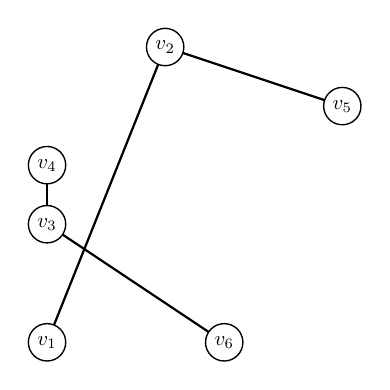
\begin{tikzpicture}[scale=0.75,transform shape]
\Vertex[x=0,y=0,L=$v_1$]{A}
\Vertex[x=2,y=5,L=$v_2$]{B}
\Vertex[x=0,y=2,L=$v_3$]{C}
\Vertex[x=0,y=3,L=$v_4$]{D}
\Vertex[x=5,y=4,L=$v_5$]{E}
\Vertex[x=3,y=0,L=$v_6$]{F}

\Edge(A)(B)
\Edge(C)(F)
\Edge(B)(E)
\Edge(C)(D)
\end{tikzpicture}

\end{center}
\end{figure}

\begin{definition}[Bipartiter Graph]
Wenn alle Knoten eines Graphen $G$ so in zwei disjunkte Mengen $S_1$ und $S_2$ (Partitionsklassen oder {\sl shores}) aufgeteilt werden können, dass keine Kanten von $G$ zwischen Knoten innerhalb derselben Shore existieren, sprechen wir von einem bipartiten Graphen.
\end{definition}

Abbildung \ref{bipartGraph} illustriert einen bipartiten Graphen mit
\[
	V = S_1 \cup S_2 = \{v_1,v_2,v_5,v_7,v_8\} \cup \{ v_3,v_4,v_6,v_9 \}
\]
und
\[
	E = \left\{  \{v_1,v_3\}, \{v_2,v_3\}, \{v_2,v_9\}, \{v_4,v_8\}, \{v_5,v_6\}, \{ v_6,v_8 \}, \{ v_7,v_9 \}  \right\}.
\]

\begin{figure}
\caption{Ein bipartiter Graph}
\label{bipartGraph}
\begin{center}

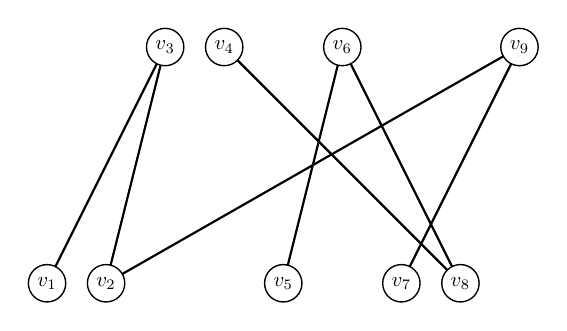
\begin{tikzpicture}[scale=0.75,transform shape]

\Vertex[x=0,y=0,L=$v_1$]{A1}
\Vertex[x=1,y=0,L=$v_2$]{A2}
\Vertex[x=2,y=4,L=$v_3$]{A3}
\Vertex[x=3,y=4,L=$v_4$]{A4}
\Vertex[x=4,y=0,L=$v_5$]{A5}
\Vertex[x=5,y=4,L=$v_6$]{A6}
\Vertex[x=6,y=0,L=$v_7$]{A7}
\Vertex[x=7,y=0,L=$v_8$]{A8}
\Vertex[x=8,y=4,L=$v_9$]{A9}

\Edge(A1)(A3)
\Edge(A2)(A3)
\Edge(A2)(A9)
\Edge(A7)(A9)
\Edge(A5)(A6)
\Edge(A6)(A8)
\Edge(A4)(A8)
\end{tikzpicture}

\end{center}
\end{figure}

\section{Zufallsgraphen}

Wenn wir Eigenschaften von vielen Graphen betrachten wollen, sind Zufallsgraphen ein hilfreicher Denkansatz. Das grundlegende Prinzip ist, eine feste Menge von Knoten $V$ anzunehmen und dann aus allen möglichen Kombinationen von Kanten (sprich aus der Potenzmenge $\mathcal{P}(E)$) mit einer definierten Wahrscheinlichkeit auszuwählen.

\bigskip
Das verbreitete Modell der Erdös-Renyi-Graphen definiert eine Klasse von Graphen $G(n, p)$ mit einer Anzahl Knoten $n$ und einer gleichverteilten Wahrscheinlichkeit $p$, dass eine Kante zwischen zwei Knoten besteht \cite{erdos}.

Da ein solcher Graph maximal $|\mathcal{P}(E)| = \binom{n}{2}$ Kanten haben kann, beträgt die Wahrscheinlichkeit, dass darin ein Graph mit genau $k$ Kanten auftritt, gegeben als
\[
\mathbb{P}(G) = p^k(1-p)^{\binom{n}{2}- k}.
\]

Es ist natürlich möglich, dass einzelne Knoten eines solchen Graphen gar keine Kanten haben, sprich das zusammenhängende Graph-Gebilde nicht alle $n$ Knoten beinhaltet. Diese Knoten werden aber trotzdem zum Graphen dazugezählt. \cite{erdos}

Abbildung \ref{pdistribution} zeigt die Auftretenswahrscheinlichkeit eines Graphen in $G(10, p)$ abhängig von der Anzahl Kanten für $p = 0.2, 0.5, 0.8.$

\begin{figure}
\caption{Verteilung der Auftretenswahrscheinlichkeit eines Zufallsgraphen}
\label{pdistribution}
\begin{center}
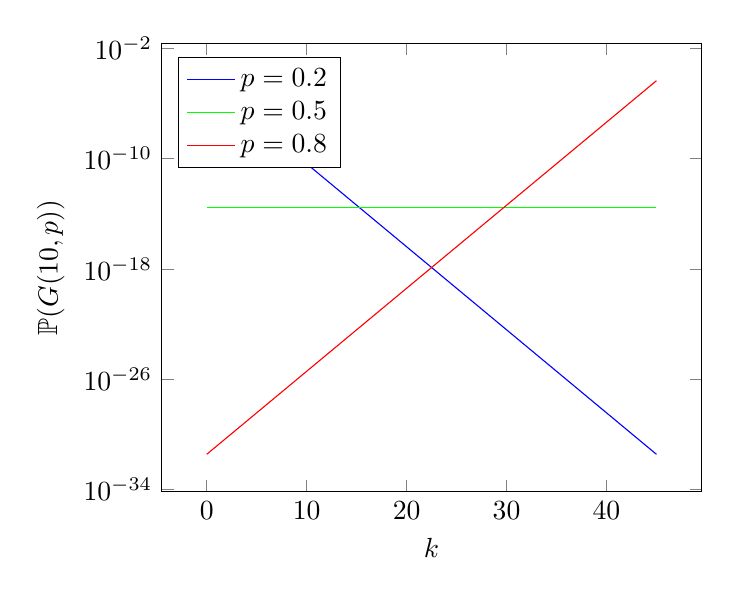
\begin{tikzpicture}
  \begin{semilogyaxis}[ 
    xlabel=$k$,
    ylabel={$\mathbb{P}(G(10, p))$},
	legend pos=north west
  ] 
    \addplot[mark=none,color=blue] coordinates {
(0,4.35561429658803E-05)
(1,1.08890357414701E-05)
(2,2.72225893536752E-06)
(3,6.8056473384188E-07)
(4,1.7014118346047E-07)
(5,4.25352958651175E-08)
(6,1.06338239662794E-08)
(7,2.65845599156984E-09)
(8,6.64613997892461E-10)
(9,1.66153499473115E-10)
(10,4.15383748682788E-11)
(11,1.03845937170697E-11)
(12,2.59614842926743E-12)
(13,6.49037107316857E-13)
(14,1.62259276829214E-13)
(15,4.05648192073035E-14)
(16,1.01412048018259E-14)
(17,2.53530120045647E-15)
(18,6.33825300114118E-16)
(19,1.58456325028529E-16)
(20,3.96140812571324E-17)
(21,9.90352031428309E-18)
(22,2.47588007857077E-18)
(23,6.18970019642693E-19)
(24,1.54742504910673E-19)
(25,3.86856262276683E-20)
(26,9.67140655691708E-21)
(27,2.41785163922927E-21)
(28,6.04462909807317E-22)
(29,1.51115727451829E-22)
(30,3.77789318629573E-23)
(31,9.44473296573934E-24)
(32,2.36118324143483E-24)
(33,5.90295810358708E-25)
(34,1.47573952589677E-25)
(35,3.68934881474193E-26)
(36,9.22337203685482E-27)
(37,2.30584300921371E-27)
(38,5.76460752303426E-28)
(39,1.44115188075857E-28)
(40,3.60287970189641E-29)
(41,9.00719925474104E-30)
(42,2.25179981368526E-30)
(43,5.62949953421315E-31)
(44,1.40737488355329E-31)
(45,3.51843720888322E-32)
	};
	\addlegendentry{$p = 0.2$}
    \addplot[mark=none,color=green] coordinates {
(0,2.8421709430404E-14)
(1,2.8421709430404E-14)
(2,2.8421709430404E-14)
(3,2.8421709430404E-14)
(4,2.8421709430404E-14)
(5,2.8421709430404E-14)
(6,2.8421709430404E-14)
(7,2.8421709430404E-14)
(8,2.8421709430404E-14)
(9,2.8421709430404E-14)
(10,2.8421709430404E-14)
(11,2.8421709430404E-14)
(12,2.8421709430404E-14)
(13,2.8421709430404E-14)
(14,2.8421709430404E-14)
(15,2.8421709430404E-14)
(16,2.8421709430404E-14)
(17,2.8421709430404E-14)
(18,2.8421709430404E-14)
(19,2.8421709430404E-14)
(20,2.8421709430404E-14)
(21,2.8421709430404E-14)
(22,2.8421709430404E-14)
(23,2.8421709430404E-14)
(24,2.8421709430404E-14)
(25,2.8421709430404E-14)
(26,2.8421709430404E-14)
(27,2.8421709430404E-14)
(28,2.8421709430404E-14)
(29,2.8421709430404E-14)
(30,2.8421709430404E-14)
(31,2.8421709430404E-14)
(32,2.8421709430404E-14)
(33,2.8421709430404E-14)
(34,2.8421709430404E-14)
(35,2.8421709430404E-14)
(36,2.8421709430404E-14)
(37,2.8421709430404E-14)
(38,2.8421709430404E-14)
(39,2.8421709430404E-14)
(40,2.8421709430404E-14)
(41,2.8421709430404E-14)
(42,2.8421709430404E-14)
(43,2.8421709430404E-14)
(44,2.8421709430404E-14)
(45,2.8421709430404E-14)
	};
	\addlegendentry{$p = 0.5$}
    \addplot[mark=none,color=red] coordinates {
(0,3.51843720888316E-32)
(1,1.40737488355326E-31)
(2,5.62949953421306E-31)
(3,2.25179981368522E-30)
(4,9.0071992547409E-30)
(5,3.60287970189636E-29)
(6,1.44115188075855E-28)
(7,5.76460752303418E-28)
(8,2.30584300921367E-27)
(9,9.2233720368547E-27)
(10,3.68934881474188E-26)
(11,1.47573952589675E-25)
(12,5.90295810358701E-25)
(13,2.36118324143481E-24)
(14,9.44473296573923E-24)
(15,3.77789318629569E-23)
(16,1.51115727451828E-22)
(17,6.04462909807311E-22)
(18,2.41785163922925E-21)
(19,9.67140655691699E-21)
(20,3.8685626227668E-20)
(21,1.54742504910672E-19)
(22,6.18970019642688E-19)
(23,2.47588007857075E-18)
(24,9.90352031428301E-18)
(25,3.96140812571321E-17)
(26,1.58456325028528E-16)
(27,6.33825300114113E-16)
(28,2.53530120045646E-15)
(29,1.01412048018258E-14)
(30,4.05648192073033E-14)
(31,1.62259276829213E-13)
(32,6.49037107316854E-13)
(33,2.59614842926741E-12)
(34,1.03845937170697E-11)
(35,4.15383748682787E-11)
(36,1.66153499473115E-10)
(37,6.64613997892459E-10)
(38,2.65845599156984E-09)
(39,1.06338239662794E-08)
(40,4.25352958651174E-08)
(41,1.7014118346047E-07)
(42,6.8056473384188E-07)
(43,2.72225893536752E-06)
(44,1.08890357414701E-05)
(45,4.35561429658803E-05)
	};
	\addlegendentry{$p = 0.8$}
  \end{semilogyaxis}
\end{tikzpicture}
\end{center}
\end{figure}

\floatname{algorithm}{Algorithmus}
\renewcommand{\algorithmicrequire}{\textbf{Eingabe:}}
\renewcommand{\algorithmicensure}{\textbf{Ausgabe:}}


\section{Generierung von Zufallsgraphen}

Zufallsgraphen zu generieren ist im Grunde genommen ziemlich einfach, wie Algorithmus~\ref{gen.naive} zeigt \cite{fastalgo}. Das Problem ist allerdings ebenfalls offensichtlich: Die Komplexitätsklasse dieses Algorithmus ist $\mathcal{O}(n^2)$.

\begin{algorithm}
\caption{Ein naiver Zufallsgraphen-Generator}
\label{gen.naive}
\begin{algorithmic}
\Require
	\Statex Anzahl Knoten $n$,
	\Statex Kantenwahrscheinlichkeit $p$.
\Ensure
	\Statex Zufallsgraph $G = (V, E)$.
\Statex
\For{$i \gets 1, n$}
\For{$j \gets i+1, n$}
\State $\theta\gets$ gleichverteilte Zufallszahl
\If{$\theta < p$}
\State $E \gets E \cup \{(v_i,v_j)\}$
\EndIf
\EndFor
\EndFor
\end{algorithmic}
\end{algorithm}


Um diese technische Suboptimalität zu lösen, verfolgen Nobari, Lu, Karras und Bressan in \cite{fastalgo} folgende Idee:

\begin{enumerate}
\item Jede Kante $(v_i, v_j)$ (und darum auch $\{v_i, v_j\}$) kann als $e_k$ ausgedrückt werden durch die Beziehungen
\[
i = \left\lfloor\frac k v \right\rfloor
\]
und
\[
j = k \mod v.
\]

\item Damit kann Algorithmus~\ref{gen.naive} $\in \mathcal{O}(n^2)$ zu einem Algorithmus mit linearer Laufzeitkomplexität $\mathcal{O}(|E|)$ umgeschrieben werden (siehe Algorithmus~\ref{gen.linear}). Da aber $|E| = \binom{n}{2}$ gilt, nützt uns das momentan noch nicht viel.

\begin{algorithm}
\caption{Ein umgeformter naiver Zufallsgraphen-Generator}
\label{gen.linear}
\begin{algorithmic}
\Require
	\Statex Kantenwahrscheinlichkeit $p$.
\Ensure
	\Statex Zufallsgraph $G = (V, E)$.
\Statex
\For{$i \gets 1, |E|$}
\State $\theta\gets$ gleichverteilte Zufallszahl
\If{$\theta < p$}
\State $E \gets E \cup \{e_i\}$
\EndIf
\EndFor
\end{algorithmic}
\end{algorithm}

\item Der eigentliche Trick folgt der Erkenntnis, dass die Wahrscheinlichkeitsverteilung einer Folge von gleichverteilten Zufallsentscheidungen, die zum selben Resultat führen, im Grunde einer geometrischen Verteilung entspricht. Dadurch können wir die Wahrscheinlichkeit, dass die nächsten $s$ Kanten des Graphen mit einer jeweiligen Wahrscheinlichkeit von $1-p$ ausgelassen werden, ausdrücken als
\[
	f(s) = p \cdot (1-p)^s,
\]
und die kumulative Verteilungsfunktion wäre (\cite{fastalgo})
\[
	F(s) = \sum\limits_{i=0}^s f(i) = 1 - (1-p)^{s+1}.
\]
Dies bedeutet, dass der Algorithmus nach jedem Setzen einer Kante eine einzige neue Zufallszahl $\alpha$ generiert, mit welcher er bestimmen kann, wieviele Kanten $s$ ausgelassen werden können (nämlich die kleinste ganze Zahl, für welche
\[
F(s) \ge \alpha
\]
gilt). Durch ein paar Takte Algebra können wir nach $s$ auflösen und bekommen eine explizite Funktion (\cite{fastalgo}):
\[
	s(\alpha) = \max(0, \left\lceil \log_{1-p}\alpha\right\rceil - 1)
\]

Damit können wir unseren Algorithmus optimieren (siehe Algorithmus~\ref{gen.opt}). Es liegt nun auf der Hand, dass dieser Algorithmus desto schneller ist, je kleiner $p$ gewählt wird. \cite{fastalgo} versucht darum, der durch die Berechnung des Logarithmus gestiegenen mathematischen Komplexität Herr zu werden, indem eine Menge an Logarithmus-Werten vorberechnet und wiederverwendet werden. Ausserdem werden noch Optimierungen vorgenommen, um den Algorithmus auf Grafik-Prozessoren laufen zu lassen. Dies ist für uns allerdings nicht weiter spannend, und darum wollen wir es bei der einfachen Optimierung wie eben gesehen belassen.

\begin{algorithm}
\caption{Ein Zufallsgraphen-Generator mit Edge Skipping}
\label{gen.opt}
\begin{algorithmic}
\Require
	\Statex Kantenwahrscheinlichkeit $p$.
\Ensure
	\Statex Zufallsgraph $G = (V, E)$.
\Statex
\Statex $i \gets -1$
\While{$i < |E|$}
\State $\alpha\gets$ gleichverteilte Zufallszahl
\State $s \gets \max(0, \left\lceil \log_{1-p}\alpha\right\rceil - 1)$
\State $i \gets i + s + 1$
\State $E \gets E \cup \{e_i\}$
\EndWhile
\State Entferne die letzte Kante
\end{algorithmic}
\end{algorithm}

\end{enumerate}

\section{Graph Coloring}

\begin{definition}[Knotenfärbung]

Für einen ungerichteten Graphen $G = (V, E)$ ist die Abbildung
\[
f : V \rightarrow C \subset \mathbb{N}
\]
eine Knotenfärbung, wenn keinen zwei Knoten, die durch eine Kante verbunden sind, dieselbe Farbe ($c \in C$) zugeordnet wird.

$G$ heisst $k$-knotenfärbbar, wenn die maximale Anzahl verwendeter Farben $k$ beträgt -- das heisst, wenn für alle $v \in V$ gilt, dass
\[
f(v) < k.
\]

Die kleinstmögliche solche Zahl $k$ wird Chromatische Zahl $\chi(G)$ geheissen.

\end{definition}

Das Auffinden einer gültigen Färbung für einen Graphen wird als Graphenfärbeproblem bezeichnet. Das dazugehörige Entscheidungsproblem, ob ein Graph $k$-färbbar ist, ist eines von Karp's 21 $\mathcal{NP}$-vollständigen Problemen \cite{hopcroft}. Praktische Anwendung finden Färbeprobleme vor allem als mathematische Formulierung von Scheduling-Problemen aller Art, beispielsweise für Stundenpläne. Ein anderes wohlstudiertes Problem ist die Frage, wie viele Farben notwendig sind, um auf einer beliebigen Landkarte jedes Land so einzufärben, dass nie zwei benachbarte Länder dieselbe Farbe haben -- mit dem lange vermuteten, aber doch überraschenden Ergebnis, dass 4 Farben ausreichend sind \cite{gonthier}.

\bigskip
Ausserdem liegt auf der Hand, dass ein bipartiter Graph stets $2$-färbbar ist.


\section{Online Graph Coloring: First Fit-Algorithmus}

Wir wollen das Graphenfärbeproblem nun als Online-Problem betrachten. Dafür stellen wir uns vor, dass der zu färbende Graph nicht komplett vorliegt, sondern jeder Knoten einzeln präsentiert wird. Jeder Knoten muss im Moment seiner Präsentation eingefärbt werden. Alle Kanten zwischen bereits aufgedeckten Knoten sind bekannt, alle anderen jedoch nicht. \cite{lovasz}

Offensichtlich kann ein solches Problem nicht per se optimal gelöst werden, da Informationen über das gesamte Problem fehlen. Abbildung~\ref{bipart.greedy} veranschaulicht den simplen First Fit-Algorithmus~\ref{algo.firstfit}:
\begin{enumerate}
\item Zuerst wird die höchste zugeordnete Farbe im Graphen gesucht ($k$) und daraus eine Menge $C'$ aufgebaut, die alle verwendeten Farben enthält.
\item Danach wird über allen Farben iteriert, und diejenigen wieder aus $C'$ entfernt, welche einem Nachbarknoten von $v$  zugeordnet sind.
\item Falls nun keine Farben mehr in $C'$ enthalten sind, wird eine neue Farbe $k+1$ erfunden und zugeordnet -- ansonsten wird die kleinste verfügbare Farbe zugeordnet.
\end{enumerate}

Wir können beobachten, wie dieser Algorithmus für einen beispielhaften (aber doch unspektakulären) bipartiten Graphen folgendermassen scheitert:
\begin{enumerate}
\item Der Knoten $v_0$ wird präsentiert, und bekommt die Farbe Blau.
\item Der Knoten $v_1$ wird präsentiert, und bekommt ebenfalls die Farbe Blau, da noch keine Kante bekannt ist.
\item Der Knoten $v_2$ wird präsentiert, und mit ihm die Kante $\{v_0, v_2\}$. $v_2$ bekommt die Farbe Rot, da $v_0$ bereits die Farbe Blau bekommen hat.
\item Der Knoten $v_3$ wird präsentiert, und mit ihm die Kanten $\{v_0, v_3\}$ und $\{v_1, v_3\}$. $v_3$ bekommt die Farbe Grün, da $v_1$ bereits die Farbe Blau und $v_2$ bereits die Farbe Rot bekommen hat.
\end{enumerate}

\begin{algorithm}
\caption{First Fit-Algorithmus für Online Graph Coloring}
\label{algo.firstfit}
\begin{algorithmic}
\Require
	\State Der präsentierte Knoten $v$,
	\State Der bereits bekannte Graph $G' = (V', E')$,
	\State Die bereits bekannte Färbung $f : V' \rightarrow C$
\Ensure
	\State Die Färbung für den präsentierten Knoten $f(v) \in C$
\Statex

\State $k \gets \max_{w \in V'}f(w)$
\State $C' \gets \{1, \dots, k \}$
\Statex
\ForAll{$c \in C'$}
\ForAll{$e \in E'$}
	\If{$v \in e$}
	\State $\{w\} \gets e \cap v$
	\If{$f(w) = c$}
		\State $C' \gets C' - \{ f(w) \}$
	\EndIf
	\EndIf
\EndFor
\EndFor

\Statex

\If{$C' \ne \{ \} $}
	\State $ f(v) \gets \min C'$
\Else
	\State $ f(v) \gets k+1$
\EndIf



\end{algorithmic}
\end{algorithm}

Der kapitale Fehler passierte bereits beim Färben von $v_1$. Es gab anhand der bereits vorhandenen Informationen keinen Grund, nicht anzunehmen, dass $v_1$ Blau zugeordnet bekommen sollte. Wenn allerdings bekannt gewesen wäre, dass $v_1$ eine Kante zu $v_3$, dieser eine Kante zu $v_2$ und dieser wiederum eine Kante zu $v_0$ haben wird, hätte dies ausgereicht, um zu erkennen, dass $v_1$ in der gegenteiligen Shore von $v_0$ hätte platziert werden müssen, wie in Abbildung~\ref{bipart.greedy.besser} illustriert wird.

\begin{figure}
\caption{Nicht optimal färbbarer bipartiter Graph}
\label{bipart.greedy}

\begin{center}
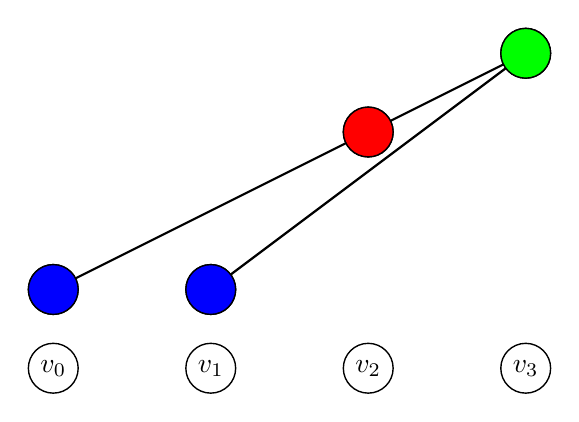
\begin{tikzpicture}[transform shape]
\Vertex[x=0,y=0,L=$v_0$]{v0}
\Vertex[x=2,y=0,L=$v_1$]{v1}
\Vertex[x=4,y=2,L=$v_2$]{v2}
\Vertex[x=6,y=3,L=$v_3$]{v3}

\AddVertexColor{blue}{v0,v1}
\AddVertexColor{red}{v2}
\AddVertexColor{green}{v3}

\Vertex[x=0,y=-1,L=$v_0$]{A}
\Vertex[x=2,y=-1,L=$v_1$]{A}
\Vertex[x=4,y=-1,L=$v_2$]{A}
\Vertex[x=6,y=-1,L=$v_3$]{A}

\Edge(v0)(v2)
\Edge(v1)(v3)
\Edge(v2)(v3)
\end{tikzpicture}


\end{center}

\end{figure}

\begin{figure}
\caption{Optimal gefärbter bipartiter Graph}
\label{bipart.greedy.besser}

\begin{center}
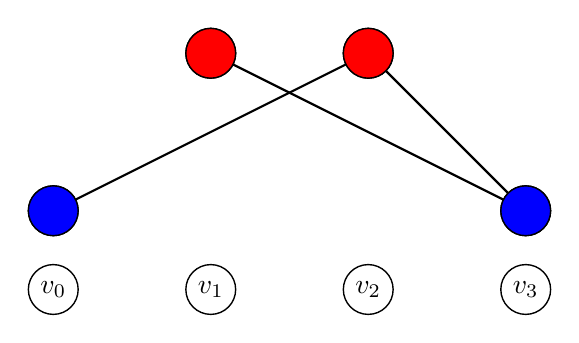
\begin{tikzpicture}[transform shape]
\Vertex[x=0,y=0,L=$v_0$]{v0}
\Vertex[x=2,y=2,L=$v_1$]{v1}
\Vertex[x=4,y=2,L=$v_2$]{v2}
\Vertex[x=6,y=0,L=$v_3$]{v3}

\AddVertexColor{blue}{v0,v3}
\AddVertexColor{red}{v2,v1}

\Vertex[x=0,y=-1,L=$v_0$]{A}
\Vertex[x=2,y=-1,L=$v_1$]{A}
\Vertex[x=4,y=-1,L=$v_2$]{A}
\Vertex[x=6,y=-1,L=$v_3$]{A}

\Edge(v0)(v2)
\Edge(v1)(v3)
\Edge(v2)(v3)
\end{tikzpicture}


\end{center}

\end{figure}

\bigskip

Das Online Coloring-Problem hat keine konstante Competitive Ratio (\cite{bipartite}), wie in \cite{gyarfas} gezeigt wird. Für den Nachvollzug wollen wir uns vergegenwärtigen, dass jeder Baum ein bipartiter Graph ist, weil alle Knoten einer Ebene nur mit Knoten der jeweiligen nächsten oder vorhergehenden Ebene verknüpft sein können, wie in Abbildung~\ref{tree} skizziert.

\begin{figure}
\caption{Ein Baum}
\label{tree}
\begin{center}
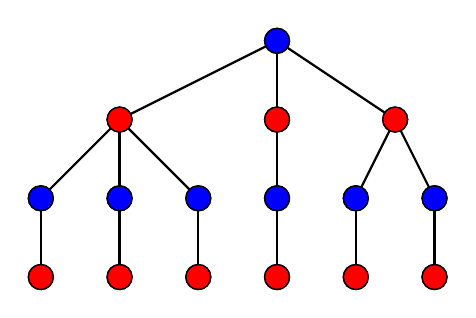
\begin{tikzpicture}[scale=0.5, transform shape]
\Vertex[x=8, y=8]{A}
\Vertex[x=4, y=6]{B}
\Vertex[x=8, y=6]{C}
\Vertex[x=11, y=6]{D}
\Vertex[x=2, y=4]{E}
\Vertex[x=4, y=4]{F}
\Vertex[x=6, y=4]{G}
\Vertex[x=8, y=4]{H}
\Vertex[x=10, y=4]{I}
\Vertex[x=12, y=4]{J}

\Vertex[x=2,y=2]{l1}
\Vertex[x=4,y=2]{l2}
\Vertex[x=6,y=2]{l3}
\Vertex[x=8,y=2]{l4}
\Vertex[x=10,y=2]{l5}
\Vertex[x=12,y=2]{l6}


\Edge(A)(B)
\Edge(A)(C)
\Edge(A)(D)

\Edge(B)(E)
\Edge(B)(F)
\Edge(B)(G)

\Edge(C)(H)

\Edge(D)(I)
\Edge(D)(J)

\Edge(E)(l1)
\Edge(F)(l2)
\Edge(G)(l3)
\Edge(H)(l4)
\Edge(I)(l5)
\Edge(J)(l6)

\AddVertexColor{blue}{A,E,F,G,H,I,J}
\AddVertexColor{red}{B,C,D,l1,l2,l3,l4,l5,l6}

\end{tikzpicture}
\end{center}
\end{figure}

Wir überlegen uns nun eine rekursive Folge von Bäumen:
\begin{itemize}
\item Der Baum $T_1$ besitzt nur einen Knoten.
\item Der Baum $T_n$ besteht aus der Vereinigung von exakten Kopien aller Bäume $T_1, \dots T_{n-1}$ sowie einem zusätzlichen Knoten, der eine Kante zu den jeweiligen Wurzelknoten all dieser Bäume hat. Abbildung~\ref{tree.rec} verdeutlicht dies.
\end{itemize}

\begin{figure}
\caption{Die Folge $T_1, \dots, T_6$}
\label{tree.rec}
\begin{center}
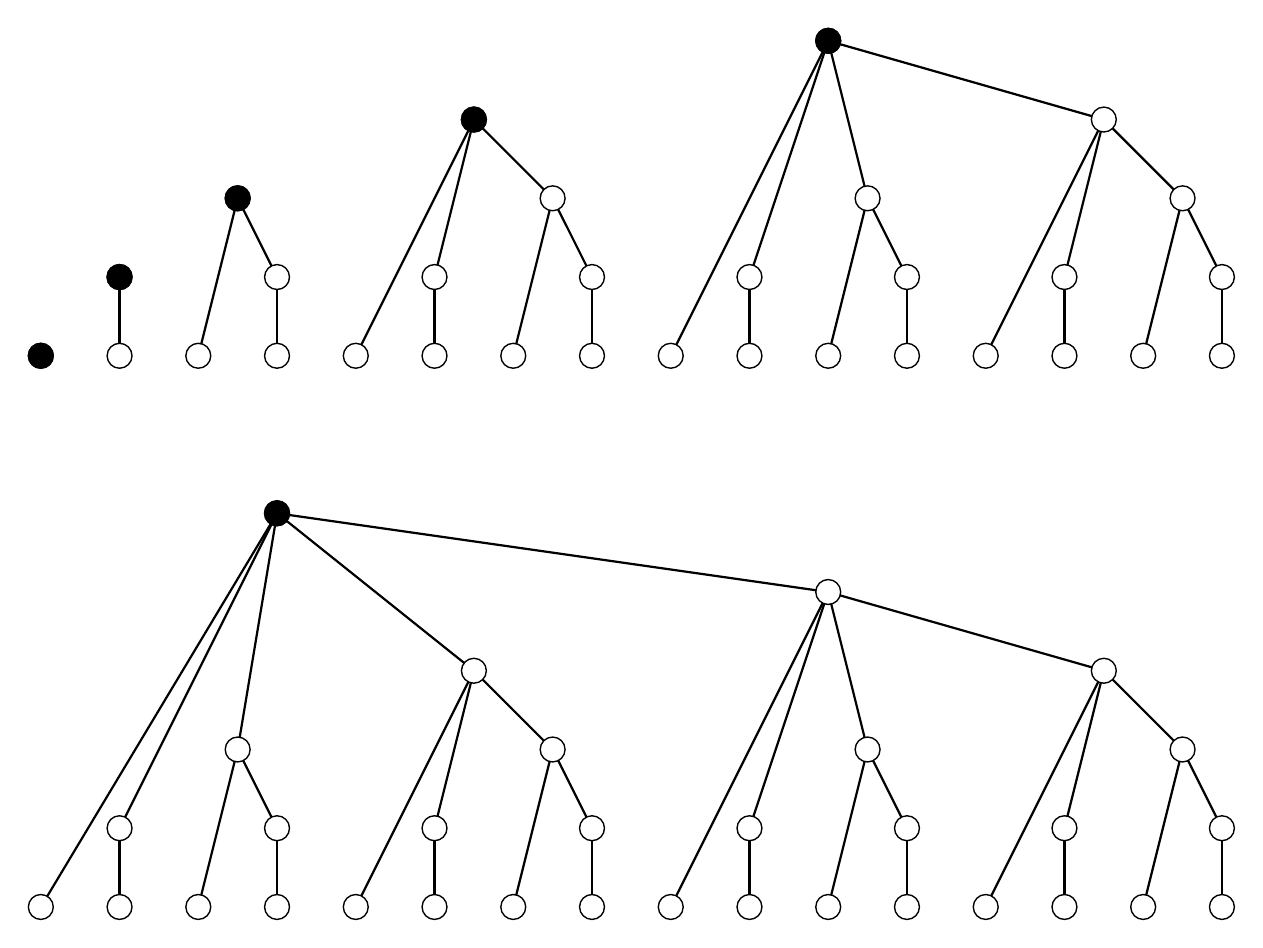
\begin{tikzpicture}[scale=0.5, transform shape]

\Vertex[x=0, y=0,L=$$]{T1x}

\Vertex[x=2, y=2,L=$$]{T2x}
\Vertex[x=2, y=0,L=$$]{T2T1x}
\Edge(T2x)(T2T1x)

\Vertex[x=4, y=0,L=$$]{T3T1x}
\Vertex[x=6, y=2,L=$$]{T3T2x}
\Vertex[x=6, y=0,L=$$]{T3T2T1x}
\Edge(T3T2x)(T3T2T1x)
\Vertex[x=5, y=4,L=$$]{T3x}
\Edge(T3T1x)(T3x)
\Edge(T3T2x)(T3x)

\Vertex[x=8, y=0,L=$$]{T4T1x}
\Vertex[x=10, y=2,L=$$]{T4T2x}
\Vertex[x=10, y=0,L=$$]{T4T2T1x}
\Edge(T4T2x)(T4T2T1x)
\Vertex[x=12, y=0,L=$$]{T4T3T1x}
\Vertex[x=14, y=2,L=$$]{T4T3T2x}
\Vertex[x=14, y=0,L=$$]{T4T3T2T1x}
\Edge(T4T3T2x)(T4T3T2T1x)
\Vertex[x=13, y=4,L=$$]{T4T3x}
\Edge(T4T3T1x)(T4T3x)
\Edge(T4T3T2x)(T4T3x)
\Vertex[x=11,y=6,L=$x$]{T4x}
\Edge(T4x)(T4T3x)
\Edge(T4x)(T4T2x)
\Edge(T4x)(T4T1x)



\Vertex[x=16, y=0,L=$$]{T5T1x}

\Vertex[x=18, y=2,L=$$]{T5T2x}
\Vertex[x=18, y=0,L=$$]{T5T2T1x}
\Edge(T5T2x)(T5T2T1x)

\Vertex[x=20, y=0,L=$$]{T5T3T1x}
\Vertex[x=22, y=2,L=$$]{T5T3T2x}
\Vertex[x=22, y=0,L=$$]{T5T3T2T1x}
\Edge(T5T3T2x)(T5T3T2T1x)
\Vertex[x=21, y=4,L=$$]{T5T3x}
\Edge(T5T3T1x)(T5T3x)
\Edge(T5T3T2x)(T5T3x)

\Vertex[x=24, y=0,L=$$]{T5T4T1x}
\Vertex[x=26, y=2,L=$$]{T5T4T2x}
\Vertex[x=26, y=0,L=$$]{T5T4T2T1x}
\Edge(T5T4T2x)(T5T4T2T1x)
\Vertex[x=28, y=0,L=$$]{T5T4T3T1x}
\Vertex[x=30, y=2,L=$$]{T5T4T3T2x}
\Vertex[x=30, y=0,L=$$]{T5T4T3T2T1x}
\Edge(T5T4T3T2x)(T5T4T3T2T1x)
\Vertex[x=29, y=4,L=$$]{T5T4T3x}
\Edge(T5T4T3T1x)(T5T4T3x)
\Edge(T5T4T3T2x)(T5T4T3x)
\Vertex[x=27,y=6,L=$$]{T5T4x}
\Edge(T5T4x)(T5T4T3x)
\Edge(T5T4x)(T5T4T2x)
\Edge(T5T4x)(T5T4T1x)

\Vertex[x=20,y=8,L=$$]{T5x}
\Edge(T5x)(T5T4x)
\Edge(T5x)(T5T3x)
\Edge(T5x)(T5T2x)
\Edge(T5x)(T5T1x)



\Vertex[x=0, y=0-14,L=$$]{T6T1x}

\Vertex[x=2, y=2-14,L=$$]{T6T2x}
\Vertex[x=2, y=0-14,L=$$]{T6T2T1x}
\Edge(T6T2x)(T6T2T1x)

\Vertex[x=4, y=0-14,L=$$]{T6T3T1x}
\Vertex[x=6, y=2-14,L=$$]{T6T3T2x}
\Vertex[x=6, y=0-14,L=$$]{T6T3T2T1x}
\Edge(T6T3T2x)(T6T3T2T1x)
\Vertex[x=5, y=4-14,L=$$]{T6T3x}
\Edge(T6T3T1x)(T6T3x)
\Edge(T6T3T2x)(T6T3x)

\Vertex[x=8, y=0-14,L=$$]{T6T4T1x}
\Vertex[x=10, y=2-14,L=$$]{T6T4T2x}
\Vertex[x=10, y=0-14,L=$$]{T6T4T2T1x}
\Edge(T6T4T2x)(T6T4T2T1x)
\Vertex[x=12, y=0-14,L=$$]{T6T4T3T1x}
\Vertex[x=14, y=2-14,L=$$]{T6T4T3T2x}
\Vertex[x=14, y=0-14,L=$$]{T6T4T3T2T1x}
\Edge(T6T4T3T2x)(T6T4T3T2T1x)
\Vertex[x=13, y=4-14,L=$$]{T6T4T3x}
\Edge(T6T4T3T1x)(T6T4T3x)
\Edge(T6T4T3T2x)(T6T4T3x)
\Vertex[x=11,y=6-14,L=$$]{T6T4x}
\Edge(T6T4x)(T6T4T3x)
\Edge(T6T4x)(T6T4T2x)
\Edge(T6T4x)(T6T4T1x)



\Vertex[x=16, y=0-14,L=$$]{T6T5T1x}

\Vertex[x=18, y=2-14,L=$$]{T6T5T2x}
\Vertex[x=18, y=0-14,L=$$]{T6T5T2T1x}
\Edge(T6T5T2x)(T6T5T2T1x)

\Vertex[x=20, y=0-14,L=$$]{T6T5T3T1x}
\Vertex[x=22, y=2-14,L=$$]{T6T5T3T2x}
\Vertex[x=22, y=0-14,L=$$]{T6T5T3T2T1x}
\Edge(T6T5T3T2x)(T6T5T3T2T1x)
\Vertex[x=21, y=4-14,L=$$]{T6T5T3x}
\Edge(T6T5T3T1x)(T6T5T3x)
\Edge(T6T5T3T2x)(T6T5T3x)

\Vertex[x=24, y=0-14,L=$$]{T6T5T4T1x}
\Vertex[x=26, y=2-14,L=$$]{T6T5T4T2x}
\Vertex[x=26, y=0-14,L=$$]{T6T5T4T2T1x}
\Edge(T6T5T4T2x)(T6T5T4T2T1x)
\Vertex[x=28, y=0-14,L=$$]{T6T5T4T3T1x}
\Vertex[x=30, y=2-14,L=$$]{T6T5T4T3T2x}
\Vertex[x=30, y=0-14,L=$$]{T6T5T4T3T2T1x}
\Edge(T6T5T4T3T2x)(T6T5T4T3T2T1x)
\Vertex[x=29, y=4-14,L=$$]{T6T5T4T3x}
\Edge(T6T5T4T3T1x)(T6T5T4T3x)
\Edge(T6T5T4T3T2x)(T6T5T4T3x)
\Vertex[x=27,y=6-14,L=$$]{T6T5T4x}
\Edge(T6T5T4x)(T6T5T4T3x)
\Edge(T6T5T4x)(T6T5T4T2x)
\Edge(T6T5T4x)(T6T5T4T1x)

\Vertex[x=20,y=8-14,L=$$]{T6T5x}
\Edge(T6T5x)(T6T5T4x)
\Edge(T6T5x)(T6T5T3x)
\Edge(T6T5x)(T6T5T2x)
\Edge(T6T5x)(T6T5T1x)

\Vertex[x=6,y=10-14,L=$x$]{T6x}

\Edge(T6x)(T6T5x)
\Edge(T6x)(T6T4x)
\Edge(T6x)(T6T3x)
\Edge(T6x)(T6T2x)
\Edge(T6x)(T6T1x)


\AddVertexColor{black}{T1x,T2x,T3x,T4x,T5x,T6x}

\end{tikzpicture}
\end{center}
\end{figure}

Wenn wir nun die Knoten dieser Bäume in einer geeigneten Reihenfolge präsentieren, maximieren wir die Menge an verdeckter Information, welche jeden Online-Algorithmus scheitern lassen wird. Für den besprochenen First Fit-Algorithmus~\ref{algo.firstfit} gehen wir beispielsweise folgendermassen vor:
\begin{enumerate}
\item Wir präsentieren zuerst alle Knoten, welche durch rekursives Kopieren von $T_1$ entstanden sind -- diese bilden auch gleichzeitig alle Blattknoten aller Bäume. Da diese Knoten natürlich keine gemeinsamen Kanten haben, wird der Algorithmus allen dieselbe Farbe zuweisen -- beispielsweise Blau.

\item Nun präsentieren wir alle Knoten, welche durch rekursives Kopieren des für $T_2$ hinzugefügten Knotens entstanden sind. (Wenn wir uns die im vorhergehenden Schritt präsentierten Knoten aus den Bäumen wegdenken würden, würden die $T_2$-originären Knoten die neue Menge an Blattknoten bilden.) Der Algorithmus kann diese Knoten nicht blau färben, da sie alle eine Kante zu schon präsentierten Knoten haben -- ergo bekommen sie die Farbe Rot.

\item Den zweiten Schritt wiederholen wir nun für die in $T_3, T_4,\dots$ hinzugefügten und in jeden weiteren Baum kopierten Knoten. Schon bei $T_3$ stellen wir fest, dass der dazumal hinzugefügte Knoten nur eine dritte Farbe zugeordnet bekommen kann, da er Kanten zu je einem der in den beiden vorangegangenen Schritten präsentierten Knoten hat.
\end{enumerate}

Die Abbildung~\ref{tree.rec.colored} veranschaulicht das Resultat. Es ist nun offensichtlich, dass der Algorithmus für jeden Baum $T_n$ genau $n$ Farben benötigt. Da jeder dieser Bäume $2^{n-1}$ Knoten hat, und es unendlich viele solcher Bäume gibt (das Spiel lässt sich bei genügend Platz und Zeit endlos weitertreiben), konstatieren wir eine nicht-konstante Competitive Ratio von
\[
	r = \frac {\log_2 k + 1} {2}
\]
in Abhängigkeit der Anzahl Knoten $k$. Gleichzeitig ist darum $\log_2 k+1$ eine untere Schranke für die minimale Anzahl Farben von Online-Algorithmen auf bipartiten Graphen -- allerdings eine zu optimistische, denn \cite{bipartite} erhöht diese auf
\[
	1.13747 \cdot \log_2 k.
\]



\begin{figure}
\caption{First Fit auf $T_1, \dots, T_6$}
\label{tree.rec.colored}
\begin{center}
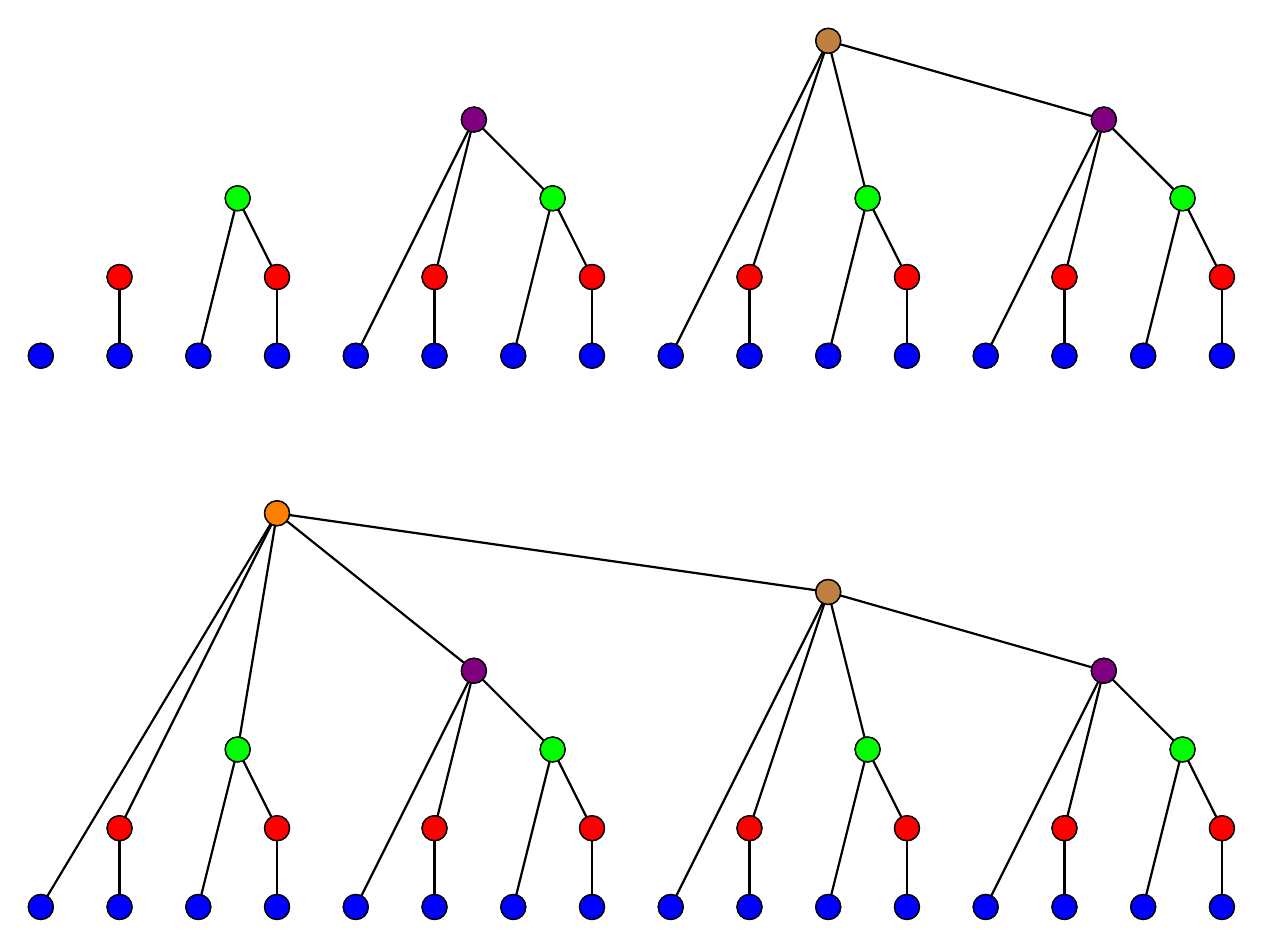
\begin{tikzpicture}[scale=0.5, transform shape]

\Vertex[x=0, y=0,L=$$]{T1x}

\Vertex[x=2, y=2,L=$$]{T2x}
\Vertex[x=2, y=0,L=$$]{T2T1x}
\Edge(T2x)(T2T1x)

\Vertex[x=4, y=0,L=$$]{T3T1x}
\Vertex[x=6, y=2,L=$$]{T3T2x}
\Vertex[x=6, y=0,L=$$]{T3T2T1x}
\Edge(T3T2x)(T3T2T1x)
\Vertex[x=5, y=4,L=$$]{T3x}
\Edge(T3T1x)(T3x)
\Edge(T3T2x)(T3x)

\Vertex[x=8, y=0,L=$$]{T4T1x}
\Vertex[x=10, y=2,L=$$]{T4T2x}
\Vertex[x=10, y=0,L=$$]{T4T2T1x}
\Edge(T4T2x)(T4T2T1x)
\Vertex[x=12, y=0,L=$$]{T4T3T1x}
\Vertex[x=14, y=2,L=$$]{T4T3T2x}
\Vertex[x=14, y=0,L=$$]{T4T3T2T1x}
\Edge(T4T3T2x)(T4T3T2T1x)
\Vertex[x=13, y=4,L=$$]{T4T3x}
\Edge(T4T3T1x)(T4T3x)
\Edge(T4T3T2x)(T4T3x)
\Vertex[x=11,y=6,L=$x$]{T4x}
\Edge(T4x)(T4T3x)
\Edge(T4x)(T4T2x)
\Edge(T4x)(T4T1x)



\Vertex[x=16, y=0,L=$$]{T5T1x}

\Vertex[x=18, y=2,L=$$]{T5T2x}
\Vertex[x=18, y=0,L=$$]{T5T2T1x}
\Edge(T5T2x)(T5T2T1x)

\Vertex[x=20, y=0,L=$$]{T5T3T1x}
\Vertex[x=22, y=2,L=$$]{T5T3T2x}
\Vertex[x=22, y=0,L=$$]{T5T3T2T1x}
\Edge(T5T3T2x)(T5T3T2T1x)
\Vertex[x=21, y=4,L=$$]{T5T3x}
\Edge(T5T3T1x)(T5T3x)
\Edge(T5T3T2x)(T5T3x)

\Vertex[x=24, y=0,L=$$]{T5T4T1x}
\Vertex[x=26, y=2,L=$$]{T5T4T2x}
\Vertex[x=26, y=0,L=$$]{T5T4T2T1x}
\Edge(T5T4T2x)(T5T4T2T1x)
\Vertex[x=28, y=0,L=$$]{T5T4T3T1x}
\Vertex[x=30, y=2,L=$$]{T5T4T3T2x}
\Vertex[x=30, y=0,L=$$]{T5T4T3T2T1x}
\Edge(T5T4T3T2x)(T5T4T3T2T1x)
\Vertex[x=29, y=4,L=$$]{T5T4T3x}
\Edge(T5T4T3T1x)(T5T4T3x)
\Edge(T5T4T3T2x)(T5T4T3x)
\Vertex[x=27,y=6,L=$$]{T5T4x}
\Edge(T5T4x)(T5T4T3x)
\Edge(T5T4x)(T5T4T2x)
\Edge(T5T4x)(T5T4T1x)

\Vertex[x=20,y=8,L=$$]{T5x}
\Edge(T5x)(T5T4x)
\Edge(T5x)(T5T3x)
\Edge(T5x)(T5T2x)
\Edge(T5x)(T5T1x)



\Vertex[x=0, y=0-14,L=$$]{T6T1x}

\Vertex[x=2, y=2-14,L=$$]{T6T2x}
\Vertex[x=2, y=0-14,L=$$]{T6T2T1x}
\Edge(T6T2x)(T6T2T1x)

\Vertex[x=4, y=0-14,L=$$]{T6T3T1x}
\Vertex[x=6, y=2-14,L=$$]{T6T3T2x}
\Vertex[x=6, y=0-14,L=$$]{T6T3T2T1x}
\Edge(T6T3T2x)(T6T3T2T1x)
\Vertex[x=5, y=4-14,L=$$]{T6T3x}
\Edge(T6T3T1x)(T6T3x)
\Edge(T6T3T2x)(T6T3x)

\Vertex[x=8, y=0-14,L=$$]{T6T4T1x}
\Vertex[x=10, y=2-14,L=$$]{T6T4T2x}
\Vertex[x=10, y=0-14,L=$$]{T6T4T2T1x}
\Edge(T6T4T2x)(T6T4T2T1x)
\Vertex[x=12, y=0-14,L=$$]{T6T4T3T1x}
\Vertex[x=14, y=2-14,L=$$]{T6T4T3T2x}
\Vertex[x=14, y=0-14,L=$$]{T6T4T3T2T1x}
\Edge(T6T4T3T2x)(T6T4T3T2T1x)
\Vertex[x=13, y=4-14,L=$$]{T6T4T3x}
\Edge(T6T4T3T1x)(T6T4T3x)
\Edge(T6T4T3T2x)(T6T4T3x)
\Vertex[x=11,y=6-14,L=$$]{T6T4x}
\Edge(T6T4x)(T6T4T3x)
\Edge(T6T4x)(T6T4T2x)
\Edge(T6T4x)(T6T4T1x)



\Vertex[x=16, y=0-14,L=$$]{T6T5T1x}

\Vertex[x=18, y=2-14,L=$$]{T6T5T2x}
\Vertex[x=18, y=0-14,L=$$]{T6T5T2T1x}
\Edge(T6T5T2x)(T6T5T2T1x)

\Vertex[x=20, y=0-14,L=$$]{T6T5T3T1x}
\Vertex[x=22, y=2-14,L=$$]{T6T5T3T2x}
\Vertex[x=22, y=0-14,L=$$]{T6T5T3T2T1x}
\Edge(T6T5T3T2x)(T6T5T3T2T1x)
\Vertex[x=21, y=4-14,L=$$]{T6T5T3x}
\Edge(T6T5T3T1x)(T6T5T3x)
\Edge(T6T5T3T2x)(T6T5T3x)

\Vertex[x=24, y=0-14,L=$$]{T6T5T4T1x}
\Vertex[x=26, y=2-14,L=$$]{T6T5T4T2x}
\Vertex[x=26, y=0-14,L=$$]{T6T5T4T2T1x}
\Edge(T6T5T4T2x)(T6T5T4T2T1x)
\Vertex[x=28, y=0-14,L=$$]{T6T5T4T3T1x}
\Vertex[x=30, y=2-14,L=$$]{T6T5T4T3T2x}
\Vertex[x=30, y=0-14,L=$$]{T6T5T4T3T2T1x}
\Edge(T6T5T4T3T2x)(T6T5T4T3T2T1x)
\Vertex[x=29, y=4-14,L=$$]{T6T5T4T3x}
\Edge(T6T5T4T3T1x)(T6T5T4T3x)
\Edge(T6T5T4T3T2x)(T6T5T4T3x)
\Vertex[x=27,y=6-14,L=$$]{T6T5T4x}
\Edge(T6T5T4x)(T6T5T4T3x)
\Edge(T6T5T4x)(T6T5T4T2x)
\Edge(T6T5T4x)(T6T5T4T1x)

\Vertex[x=20,y=8-14,L=$$]{T6T5x}
\Edge(T6T5x)(T6T5T4x)
\Edge(T6T5x)(T6T5T3x)
\Edge(T6T5x)(T6T5T2x)
\Edge(T6T5x)(T6T5T1x)

\Vertex[x=6,y=10-14,L=$x$]{T6x}

\Edge(T6x)(T6T5x)
\Edge(T6x)(T6T4x)
\Edge(T6x)(T6T3x)
\Edge(T6x)(T6T2x)
\Edge(T6x)(T6T1x)


\AddVertexColor{blue}{T1x,T2T1x,T3T1x,T3T2T1x, T4T1x,T4T2T1x,T4T3T1x,T4T3T2T1x}
\AddVertexColor{blue}{T5T1x,T5T2T1x,T5T3T1x,T5T3T2T1x, T5T4T1x,T5T4T2T1x,T5T4T3T1x,T5T4T3T2T1x}

\AddVertexColor{blue}{T6T1x,T6T2T1x,T6T3T1x,T6T3T2T1x, T6T4T1x,T6T4T2T1x,T6T4T3T1x,T6T4T3T2T1x}
\AddVertexColor{blue}{T6T5T1x,T6T5T2T1x,T6T5T3T1x,T6T5T3T2T1x, T6T5T4T1x,T6T5T4T2T1x,T6T5T4T3T1x,T6T5T4T3T2T1x}

\AddVertexColor{red}{T2x}
\AddVertexColor{red}{T3T2x}
\AddVertexColor{red}{T4T3T2x,T4T2x}
\AddVertexColor{red}{T5T4T3T2x,T5T4T2x,T5T3T2x,T5T2x}
\AddVertexColor{red}{T6T5T4T3T2x,T6T5T4T2x,T6T5T3T2x,T6T5T2x,T6T4T3T2x,T6T4T2x,T6T3T2x,T6T2x}

\AddVertexColor{green}{T3x}
\AddVertexColor{green}{T4T3x}
\AddVertexColor{green}{T5T4T3x,T5T3x}
\AddVertexColor{green}{T6T5T4T3x,T6T5T3x,T6T4T3x,T6T3x}

\AddVertexColor{violet}{T4x}
\AddVertexColor{violet}{T5T4x}
\AddVertexColor{violet}{T6T5T4x,T6T4x}

\AddVertexColor{brown}{T5x,T6T5x}

\AddVertexColor{orange}{T6x}


\end{tikzpicture}
\end{center}
\end{figure}


\chapter{Online Coloring von bipartiten Graphen mit Advice}

Im vorhergehenden Kapitel haben wir festgestellt, dass Online Coloring auf bipartiten Graphen nicht kompetitiv ist. Wir wollen nun betrachten, wie sich der Einsatz eines Orakels im Sinne der Advice Complexity auf die Kompetivität auswirken würde -- und hoffen auf ähnlich erstaunliche Ergebnisse wie im Falle von {\sc SimpleKnapsack}.

\section{Online Coloring Algorithmus mit Advice}

\bigskip
Das Hauptproblem von Online-Färbe-Algorithmen scheint zu sein, dass es Situationen während der Präsentation der Knoten geben kann, welche zu gleichen Färbungen von Knoten auf beiden Shores führen können, wie wir durch Betrachten der Abbildungen~\ref{bipart.greedy} und \ref{bipart.greedy.besser} rekapitulieren können. Dies ist einzig der fehlenden Information über die Zukunft geschuldet. Ein allenfalls eingesetztes Orakel sollte also in genau diesem Aspekt helfen können. Die benötigte Unterstützung beschränkt sich aber auf ein schmales Band: um eine konstante Competitive Ratio $\frac k 2$ zu erreichen (sprich: $k$ Farben zuzulassen), ist einzig wichtig, die Farben $k$ und $k-1$ nicht durcheinander zu bringen \cite{bipartite}.

\bigskip
Dies führt zum Algorithmus~\ref{algo.advice}, welcher wie der First Fit-Algorithmus immer die niedrigstmögliche Farbe zuordnet. Falls aber für einen Knoten die einzigen beiden möglichen Farben $k-1$ und $k$ sind, fragt er das Orakel, wie der Knoten gefärbt werden soll. Damit wird sichergestellt, dass alle Knoten mit der Farbe $k-1$ auf der einen Seite und alle Knoten mit der Farbe $k$ auf der anderen Seite des Graphen sind.

\begin{algorithm}
\caption{Online Graph Coloring-Algorithmus mit Advice}
\label{algo.advice}
\begin{algorithmic}
\Require
	\State Der präsentierte Knoten $v$,
	\State Der bereits bekannte Graph $G' = (V', E')$,
	\State Die bereits bekannte Färbung $f : V' \rightarrow C$,
	\State Die maximale Anzahl erlaubter Farben $k$,
	\State Das Orakel $\mathcal{O} : V \rightarrow \{0,1\}$
\Ensure
	\State Die Färbung für den präsentierten Knoten $f(v) \in C$
\Statex

\State $C' \gets \{1, \dots, k\}$
\ForAll{$c \in C'$}
\ForAll{$e \in E'$}
	\If{$v \in e$}
	\State $\{w\} \gets e \cap v$
	\If{$f(w) = c$}
		\State $C' \gets C' - \{ f(w) \}$
	\EndIf
	\EndIf
\EndFor
\EndFor

\Statex

\If{$C' \ne \{k-1,k\}$}
	\State $ f(v) \gets \min C'$
\Else
	\State $ f(v) \gets k-1+\mathcal{O}(v)$
\EndIf

\end{algorithmic}
\end{algorithm}

\section{Obere und untere Schranken für Advice Bits}

Bezüglich den Schranken für Advice Bits lassen sich folgende Aussagen machen:

\begin{itemize}
\item Um jeden bipartiten Graphen mit $n$ Knoten optimal färben zu können, sind höchstens $n-2$ Advice Bits nötig. Die Begründung liegt darin, dass ein Algorithmus konstruiert werden kann, der folgendermassen funktioniert:

\begin{enumerate}
\item Der erste Knoten bekommt die Farbe $1$.
\item Bei der Präsentation des zweiten Knotens wird das Orakel gefragt, ob jedem bei der Präsentation isolierten Knoten ebenfalls die Farbe $1$ zugeordnet werden soll. Nicht-isolierte Knoten bekommen die bezüglich des Nachbarknoten entgegengesetzte Farbe. Bei einer Bejahung dieser Frage beträgt die Anzahl Advice Bits genau $1 \le n-2$.
\item Falls das Orakel bei Schritt 2 verneint, wird es bei jedem isolierten Knoten nach der Farbe gefragt. Das Orakel würde die erste Frage aber nur verneinen, wenn es mindestens $2$ nicht isolierte Knoten gibt -- ansonsten wäre Optimalität auch noch gewährleistet, wenn die Farbe $1$ auf beiden Shores auftauchen würde. Also beträgt die Anzahl Advice Bits höchstens $n-2$. \cite{bipartite}
\end{enumerate}

\item Um jeden bipartiten Graphen mit $n$ Knoten optimal färben zu können, sind mindestens $n-3$ Advice Bits nötig. \cite{bipartite}

\item Um jeden bipartiten Graphen mit $n$ Knoten mit höchstens $k > 2$ Farben färben zu können, sind höchstens
$\frac{n} { \sqrt{2^{k-1}}}$
Advice Bits nötig \cite{bipartite}. Dies ergibt sich aus der Beobachtung, dass die Befragung des Orakels, ob die Farbe $k$ oder $k-1$ zugewiesen werden soll, nur jeweils notwendig wird, wenn der aktuell präsentierte Knoten $k-2$ Kanten zu Nachbarn mit genau den Farben $\{1,\dots, k-2\}$ hat. Durch Induktion lässt sich dann zeigen, dass dies nur für jeden $ \sqrt{2^{k-1}}$ten aller $n$ Knoten der Fall ist \cite{bipartite, trotter}.

\bigskip
Wir könnten entgegenhalten, dass wir einen Graphen konstruieren könnten, der für diesen Algorithmus möglichst schlecht funktioniert, indem wir die Anzahl an $\{k-1, k\}$-Auswahlmöglichkeit maximieren. Dies könnte zum Beispiel durch die Konstruktion von Bäumen $T_1, \dots T_{k-2}$ erreicht werden, welche nicht miteinander verbunden sind. Die Präsentation dieser Bäume führte dazu, dass der Algorithmus für den jeweiligen originären Knoten des $i$ten Baumes die Farbe $i$ verwenden müsste. Die restlichen $n - 1 + 2^{k-1}$ Knoten würden dann mit all diesen originären Baumknoten verbunden und präsentiert. Da der Algorithmus für die Nachbarn dieser Knoten bereits $k-2$ Farben verwendet hätte, müsste er die Farbe $k-1$ oder $k$ verwenden -- was zu $n - 1 + 2^{k-1}$  Advice Bits führen würde.

\bigskip
Dies ist allerdings nur vordergründig ein Problem, da $k$ nur die Höchstgrenze an erlaubten Farben darstellt. Tatsächlich ist es so, dass die Anzahl Advice Bits für einen derartigen Graphen bei $k' = k-1$ ausserordentlich klein wird (weil der Adversary seine gesamte Konzentration in die Forcierung von $k-2$ legt).


\end{itemize}


\section{Experimente}

Mit Hilfe des zu dieser Arbeit gehörenden Programms {\tt GraphBonanza} werden wir nun einige Experimente durchführen. Die aus den Experimenten angefallenen Daten sind von \url{https://github.com/foyan/GraphBonanza/blob/master/doc/thesis/Experimente.xlsx} beziehbar.

\subsection{Anzahl Advice Bits für dieselbe Competitive Ratio wie First Fit}

In diesem ersten Experiment wollen wir untersuchen, wie viele Advice Bits durchschnittlich, minimal und maximal benötigt werden, um eine repräsentative Menge von $G(n,p)$-Graphen zu färben. Dabei wird die maximale Anzahl Farben $k$ für den Algorithmus mit Advice so gewählt, dass er jeweils dem Resultat von First Fit entspricht. Tabelle~\ref{tab.exp1p01} zeigt das Resultat für 10000 Instanzen von $G(n = 1000, p = 0.1)$. Die Daten sind über die vom First Fit-Algorithmus benötigten Anzahl Farben gruppiert (Spalte FF: \# colors) und weisen die minimale, maximale und durchschnittliche Anzahl Advice Bits aus, welche der Algorithmus mit Advice angefragt hat. Die Tabellen~\ref{tab.exp1p05} und \ref{tab.exp1p09} zeigen die Resultate desselben Experiments für $p = 0.5$ respektive $p = 0.9$.

\bigskip
Des weiteren geben die Abbildungen~\ref{fig.exp1.1}, \ref{fig.exp1.2}, \ref{fig.exp1.3} einen visuellen Überblick über diesen Sachverhalt. Dabei zeigt die rote Kurve den Verlauf der oberen Schranke, der graue Bereich die jeweilige Bandbreite der verwendeten Advice Bits, die schwarze Kurve den durchschnittliche Anzahl Advice Bits sowie die blauen Balken die Anzahl Male, für welche der First Fit-Algorithmus die entsprechende Anzahl Farben verwendet hat.

\begin{table}
\caption{First Fit gegen Algorithmus mit Advice für 10000 Instanzen von $G(1000, 0.1)$}
\label{tab.exp1p01}

% Table generated by Excel2LaTeX from sheet 'Sheet1'

  \centering
    \begin{tabular}{rrrrr}
    \toprule
    {\tt{FF}}: \# colors & \# samples & {\tt{AA}}: min advice bits & {\tt{AA}}: avg advice bits & {\tt{AA}}: max advice bits \\
    \midrule
2     & 11    & 13    & 17.72727273 & 26 \\
3     & 156   & 18    & 46.90384615 & 156 \\
4     & 199   & 17    & 54.11055276 & 186 \\
5     & 222   & 14    & 51.38288288 & 175 \\
6     & 255   & 10    & 42.21176471 & 123 \\
7     & 382   & 3     & 30.23036649 & 115 \\
8     & 661   & 1     & 19.28290469 & 87 \\
9     & 1087  & 1     & 15.05335787 & 62 \\
10    & 1570  & 1     & 12.19235669 & 44 \\
11    & 1756  & 1     & 10.90261959 & 31 \\
12    & 1577  & 1     & 10.10653139 & 22 \\
13    & 1122  & 0     & 8.163101604 & 15 \\
14    & 642   & 0     & 5.230529595 & 11 \\
15    & 260   & 0     & 2.384615385 & 7 \\
16    & 88    & 0     & 1.579545455 & 5 \\
17    & 12    & 0     & 0.5   & 3 \\

    \bottomrule
    \end{tabular}%

\end{table}

\begin{table}
\caption{First Fit gegen Algorithmus mit Advice für 10000 Instanzen von $G(1000, 0.5)$}
\label{tab.exp1p05}
  \centering
% Table generated by Excel2LaTeX from sheet 'Sheet1'
    \begin{tabular}{rrrrr}
    \toprule
    {\tt{FF}}: \# colors & \# samples & {\tt{AA}}: min advice bits & {\tt{AA}}: avg advice bits & {\tt{AA}}: max advice bits \\
    \midrule
2     & 4190  & 1     & 3.999045346 & 16 \\
3     & 3040  & 1     & 5.537171053 & 23 \\
4     & 1474  & 1     & 5.865671642 & 34 \\
5     & 708   & 1     & 6.015536723 & 34 \\
6     & 330   & 1     & 6.387878788 & 32 \\
7     & 137   & 1     & 6.510948905 & 27 \\
8     & 63    & 1     & 6.587301587 & 25 \\
9     & 31    & 1     & 7.064516129 & 19 \\
10    & 17    & 2     & 6.117647059 & 13 \\
11    & 7     & 2     & 4.285714286 & 10 \\
12    & 2     & 3     & 3.5   & 4 \\
13    & 1     & 2     & 2     & 2 \\


    \bottomrule
    \end{tabular}%

\end{table}

\begin{table}
\caption{First Fit gegen Algorithmus mit Advice für 10000 Instanzen von $G(1000, 0.9)$}
\label{tab.exp1p09}
  \centering
% Table generated by Excel2LaTeX from sheet 'Sheet1'
\begin{tabular}{rrrrr}
\toprule
    {\tt{FF}}: \# colors & \# samples & {\tt{AA}}: min advice bits & {\tt{AA}}: avg advice bits & {\tt{AA}}: max advice bits \\
\midrule
2     & 9035  & 1     & 2.221140011 & 155 \\
3     & 905   & 1     & 2.722651934 & 13 \\
4     & 58    & 1     & 2.793103448 & 8 \\
5     & 2     & 3     & 4.5   & 6 \\
\bottomrule
\end{tabular}%


\end{table}

\begin{figure}
\caption{{\tt{FF}} gegen {\tt{AA}} für 10000 Instanzen von $G(1000, p)$, I}
\label{fig.exp1.1}
\centering

\subfloat[$p = 0.01$]

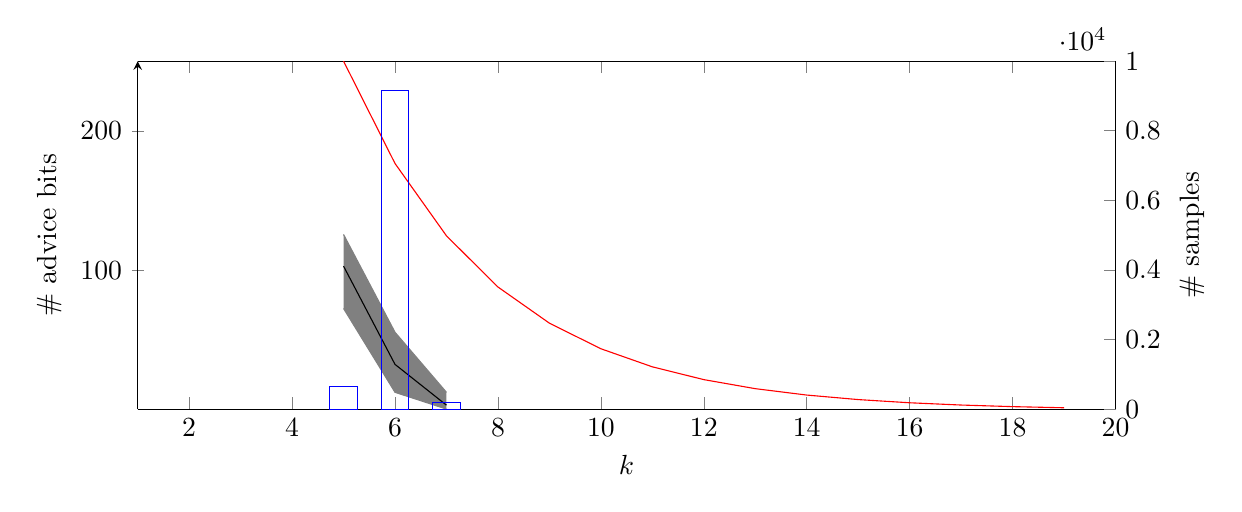
\begin{tikzpicture}
  \begin{axis}[ 
    xlabel=$k$,
    ylabel={\# advice bits},
legend pos=north west, xmin=1,xmax=20, height=6cm,width=14cm, axis y line=left
  ] 
    \addplot[mark=none,color=gray, stack plots=y] coordinates {
(5,73)
(6,13)
(7,1)


	};

    \addplot[mark=none,fill=gray,draw=none, stack plots=y] coordinates {
(5,53)
(6,43)
(7,12)



	} \closedcycle;

    \addplot[mark=none,color=gray] coordinates {
(5,126)
(6,56)
(7,13)



	};

\addplot[color=black] coordinates {
(5,103.3)
(6,33)
(7,3.8)


};

\addplot[color=red] coordinates {

(5,250)
(6,176.776695296637)
(7,125)
(8,88.3883476483184)
(9,62.5)
(10,44.1941738241592)
(11,31.25)
(12,22.0970869120796)
(13,15.625)
(14,11.0485434560398)
(15,7.8125)
(16,5.5242717280199)
(17,3.90625)
(18,2.76213586400995)
(19,1.953125)



};

  \end{axis}

\begin{axis}[
height=6cm,width=14cm,
      xmin = 1, xmax = 20,
      ymin = 0, ymax = 10000,
      hide x axis,
      axis y line*=right,
      ylabel={\# samples},
      ylabel near ticks, ybar
    ]
      \addplot[blue] coordinates {
(5,646)
(6,9162)
(7,192)





	};
    \end{axis}
\end{tikzpicture}


\subfloat[$p = 0.02$]

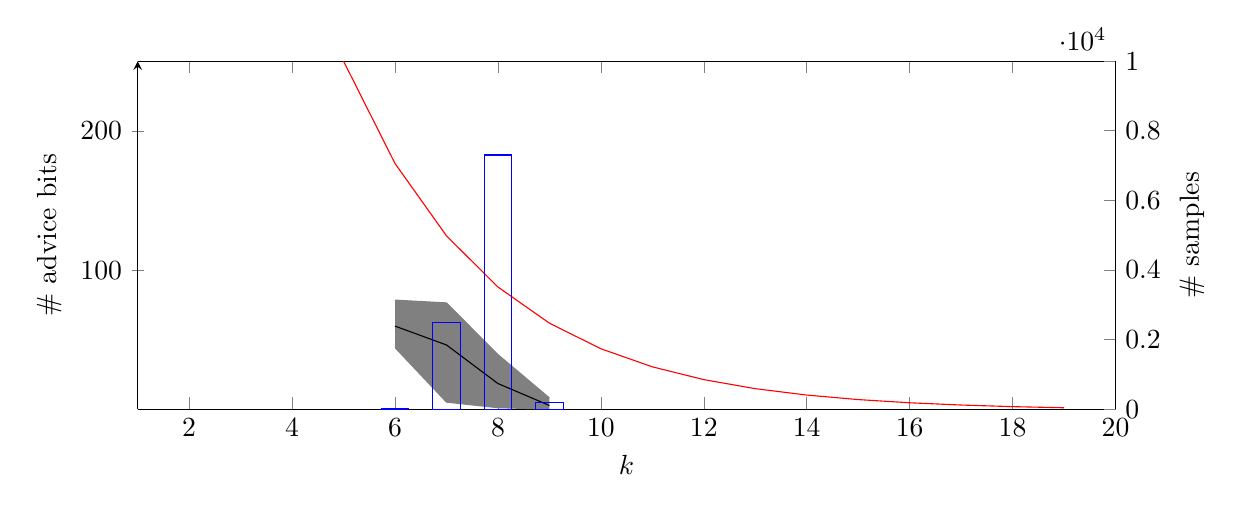
\begin{tikzpicture}
  \begin{axis}[ 
    xlabel=$k$,
    ylabel={\# advice bits},
	legend pos=north west, xmin=1,xmax=20, height=6cm,width=14cm, axis y line=left
  ] 
    \addplot[mark=none,color=gray, stack plots=y] coordinates {
(6,45)
(7,6)
(8,2)
(9,1)


	};

    \addplot[mark=none,fill=gray,draw=none, stack plots=y] coordinates {
(6,34)
(7,71)
(8,38)
(9,8)



	} \closedcycle;

    \addplot[mark=none,color=gray] coordinates {
(6,79)
(7,77)
(8,40)
(9,9)



	};

\addplot[color=black] coordinates {
(6,60.4)
(7,46.9)
(8,19.3)
(9,3.6)


};

\addplot[color=red] coordinates {

(5,250)
(6,176.776695296637)
(7,125)
(8,88.3883476483184)
(9,62.5)
(10,44.1941738241592)
(11,31.25)
(12,22.0970869120796)
(13,15.625)
(14,11.0485434560398)
(15,7.8125)
(16,5.5242717280199)
(17,3.90625)
(18,2.76213586400995)
(19,1.953125)



};

  \end{axis}

\begin{axis}[
height=6cm,width=14cm,
      xmin = 1, xmax = 20,
      ymin = 0, ymax = 10000,
      hide x axis,
      axis y line*=right,
      ylabel={\# samples},
      ylabel near ticks, ybar
    ]
      \addplot[blue] coordinates {
(6,15)
(7,2501)
(8,7302)
(9,182)




	};
    \end{axis}
\end{tikzpicture}


\subfloat[$p = 0.05$]

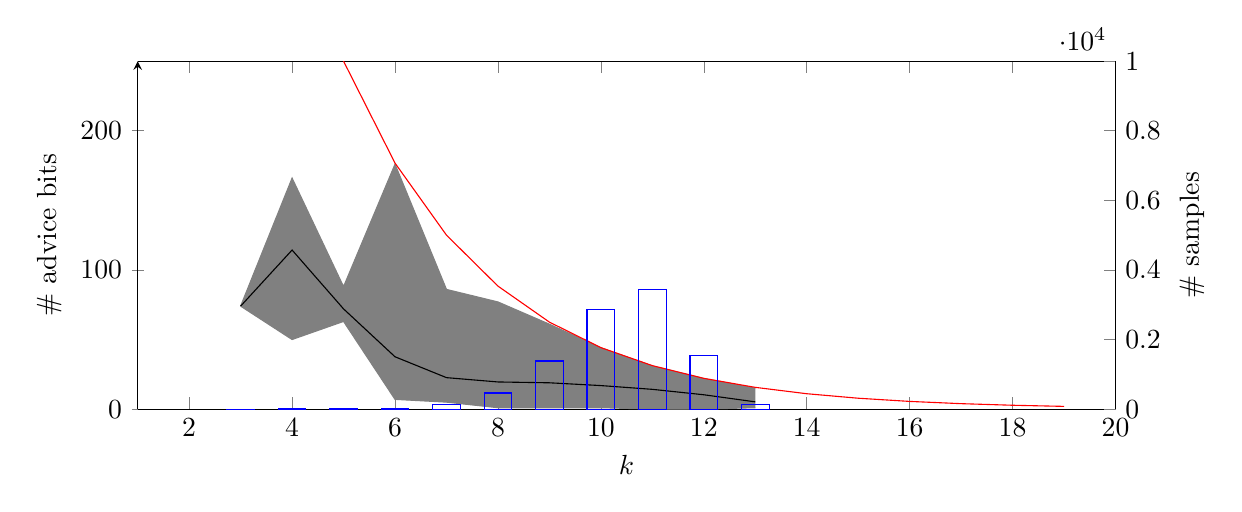
\begin{tikzpicture}
  \begin{axis}[ 
    xlabel=$k$,
    ylabel={\# advice bits},
	legend pos=north west, xmin=1,xmax=20, height=6cm,width=14cm, axis y line=left
  ] 
    \addplot[mark=none,color=gray, stack plots=y] coordinates {
(3,74)
(4,50)
(5,63)
(6,7)
(7,5)
(8,1)
(9,1)
(10,1)
(11,0)
(12,0)
(13,1)




	};

    \addplot[mark=none,fill=gray,draw=none, stack plots=y] coordinates {
(3,0)
(4,116)
(5,25)
(6,169)
(7,81)
(8,76)
(9,60)
(10,43)
(11,31)
(12,22)
(13,14)





	} \closedcycle;

    \addplot[mark=none,color=gray] coordinates {
(3,74)
(4,166)
(5,88)
(6,176)
(7,86)
(8,77)
(9,61)
(10,44)
(11,31)
(12,22)
(13,15)





	};

\addplot[color=black] coordinates {
(3,74)
(4,114.3)
(5,72)
(6,37.6)
(7,22.6)
(8,19.5)
(9,18.9)
(10,16.9)
(11,14.2)
(12,10.3)
(13,5.2)




};

\addplot[color=red] coordinates {

(5,250)
(6,176.776695296637)
(7,125)
(8,88.3883476483184)
(9,62.5)
(10,44.1941738241592)
(11,31.25)
(12,22.0970869120796)
(13,15.625)
(14,11.0485434560398)
(15,7.8125)
(16,5.5242717280199)
(17,3.90625)
(18,2.76213586400995)
(19,1.953125)



};

  \end{axis}

\begin{axis}[
height=6cm,width=14cm,
      xmin = 1, xmax = 20,
      ymin = 0, ymax = 10000,
      hide x axis,
      axis y line*=right,
      ylabel={\# samples},
      ylabel near ticks, ybar 
    ]
      \addplot[blue] coordinates {
(3,1)
(4,3)
(5,3)
(6,25)
(7,139)
(8,462)
(9,1381)
(10,2868)
(11,3430)
(12,1553)
(13,135)






	};
    \end{axis}
\end{tikzpicture}


\end{figure}

\begin{figure}
\caption{{\tt{FF}} gegen {\tt{AA}} für 10000 Instanzen von $G(1000, p)$, II}
\label{fig.exp1.2}
\centering

\subfloat[$p = 0.1$]

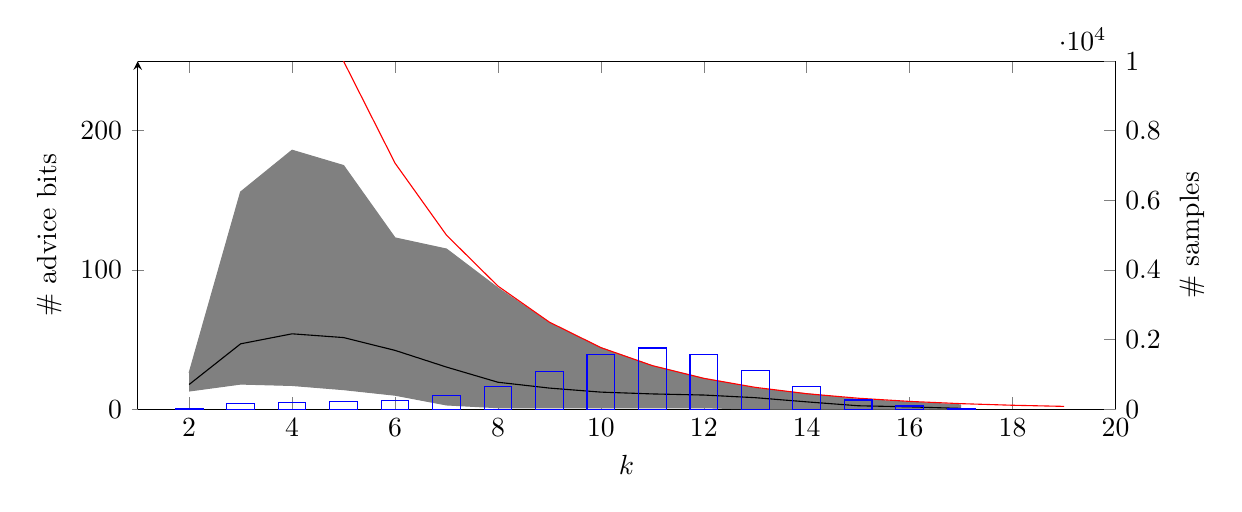
\begin{tikzpicture}
  \begin{axis}[ 
    xlabel=$k$,
    ylabel={\# advice bits},
	legend pos=north west, xmin=1,xmax=20, height=6cm,width=14cm, axis y line=left
  ] 
    \addplot[mark=none,color=gray, stack plots=y] coordinates {
(2,13)
(3,18)
(4,17)
(5,14)
(6,10)
(7,3)
(8,1)
(9,1)
(10,1)
(11,1)
(12,1)
(13,0)
(14,0)
(15,0)
(16,0)
(17,0)


	};

    \addplot[mark=none,fill=gray,draw=none, stack plots=y] coordinates {
(2,13)
(3,138)
(4,169)
(5,161)
(6,113)
(7,112)
(8,86)
(9,61)
(10,43)
(11,30)
(12,21)
(13,15)
(14,11)
(15,7)
(16,5)
(17,3)



	} \closedcycle;

    \addplot[mark=none,color=gray] coordinates {
(2,26)
(3,156)
(4,186)
(5,175)
(6,123)
(7,115)
(8,87)
(9,62)
(10,44)
(11,31)
(12,22)
(13,15)
(14,11)
(15,7)
(16,5)
(17,3)



	};

\addplot[color=black] coordinates {
(2,17.7)
(3,46.9)
(4,54.1)
(5,51.4)
(6,42.2)
(7,30.2)
(8,19.3)
(9,15.1)
(10,12.2)
(11,10.9)
(12,10.1)
(13,8.2)
(14,5.2)
(15,2.4)
(16,1.6)
(17,0.5)


};



\addplot[color=red] coordinates {

(5,250)
(6,176.776695296637)
(7,125)
(8,88.3883476483184)
(9,62.5)
(10,44.1941738241592)
(11,31.25)
(12,22.0970869120796)
(13,15.625)
(14,11.0485434560398)
(15,7.8125)
(16,5.5242717280199)
(17,3.90625)
(18,2.76213586400995)
(19,1.953125)



};

  \end{axis}
\begin{axis}[
height=6cm,width=14cm,
      xmin = 1, xmax = 20,
      ymin = 0, ymax = 10000,
      hide x axis,
      axis y line*=right,
      ylabel={\# samples},
      ylabel near ticks, ybar
    ]
      \addplot[blue] coordinates {
(2,11)
(3,156)
(4,199)
(5,222)
(6,255)
(7,382)
(8,661)
(9,1087)
(10,1570)
(11,1756)
(12,1577)
(13,1122)
(14,642)
(15,260)
(16,88)
(17,12)




	};
    \end{axis}
\end{tikzpicture}

\subfloat[$p = 0.2$]

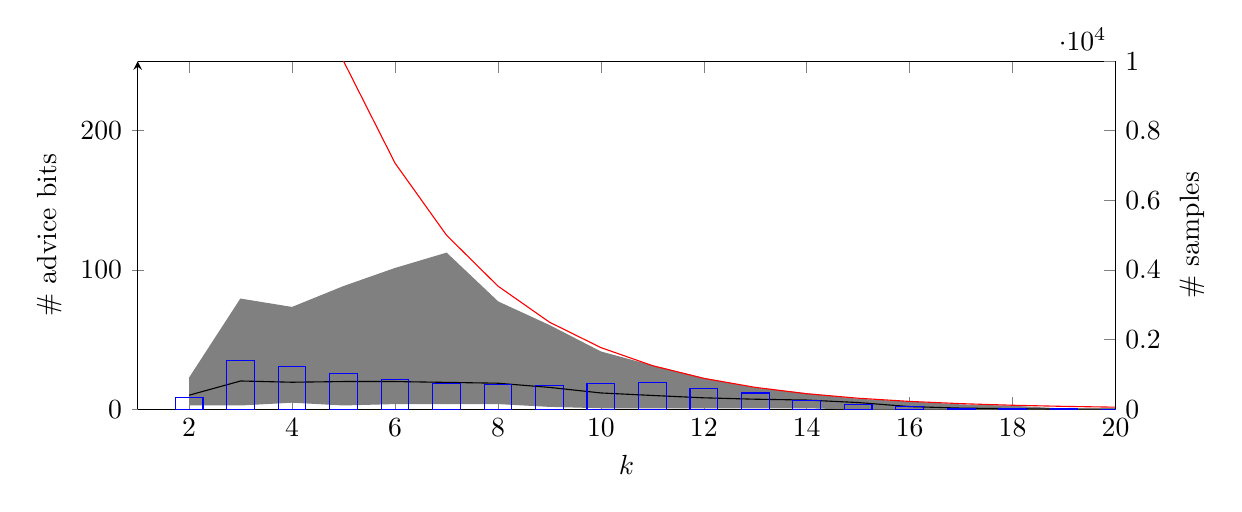
\begin{tikzpicture}
  \begin{axis}[ 
    xlabel=$k$,
    ylabel={\# advice bits},
	legend pos=north west, xmin=1,xmax=20, height=6cm,width=14cm, axis y line=left
  ] 
    \addplot[mark=none,color=gray, stack plots=y] coordinates {
(2,3)
(3,3)
(4,5)
(5,3)
(6,4)
(7,4)
(8,4)
(9,2)
(10,1)
(11,1)
(12,1)
(13,1)
(14,1)
(15,0)
(16,0)
(17,0)
(18,0)
(19,0)
(20,0)


	};

    \addplot[mark=none,fill=gray,draw=none, stack plots=y] coordinates {
(2,19)
(3,76)
(4,68)
(5,85)
(6,97)
(7,108)
(8,73)
(9,58)
(10,40)
(11,30)
(12,21)
(13,14)
(14,10)
(15,7)
(16,5)
(17,3)
(18,2)
(19,0)
(20,0)



	} \closedcycle;

    \addplot[mark=none,color=gray] coordinates {
(2,22)
(3,79)
(4,73)
(5,88)
(6,101)
(7,112)
(8,77)
(9,60)
(10,41)
(11,31)
(12,22)
(13,15)
(14,11)
(15,7)
(16,5)
(17,3)
(18,2)
(19,0)
(20,0)




	};

\addplot[color=black] coordinates {
(2,10)
(3,20.2)
(4,19.3)
(5,19.8)
(6,19.8)
(7,19.2)
(8,18.6)
(9,15.6)
(10,11.6)
(11,9.8)
(12,8.1)
(13,7.1)
(14,6.5)
(15,4.7)
(16,1.8)
(17,0.7)
(18,0.3)
(19,0)
(20,0)



};

\addplot[color=red] coordinates {

(5,250)
(6,176.776695296637)
(7,125)
(8,88.3883476483184)
(9,62.5)
(10,44.1941738241592)
(11,31.25)
(12,22.0970869120796)
(13,15.625)
(14,11.0485434560398)
(15,7.8125)
(16,5.5242717280199)
(17,3.90625)
(18,2.76213586400995)
(19,1.953125)
(20,1.38106793200498)



};


  \end{axis}

\begin{axis}[
height=6cm,width=14cm,
      xmin = 1, xmax = 20,
      ymin = 0, ymax = 10000,
      hide x axis,
      axis y line*=right,
      ylabel={\# samples},
      ylabel near ticks, ybar
    ]
      \addplot[blue] coordinates {
(2,332)
(3,1403)
(4,1217)
(5,1036)
(6,842)
(7,735)
(8,706)
(9,678)
(10,747)
(11,757)
(12,601)
(13,463)
(14,248)
(15,135)
(16,68)
(17,23)
(18,6)
(19,2)
(20,1)





	};
    \end{axis}

\end{tikzpicture}

\subfloat[$p = 0.3$]

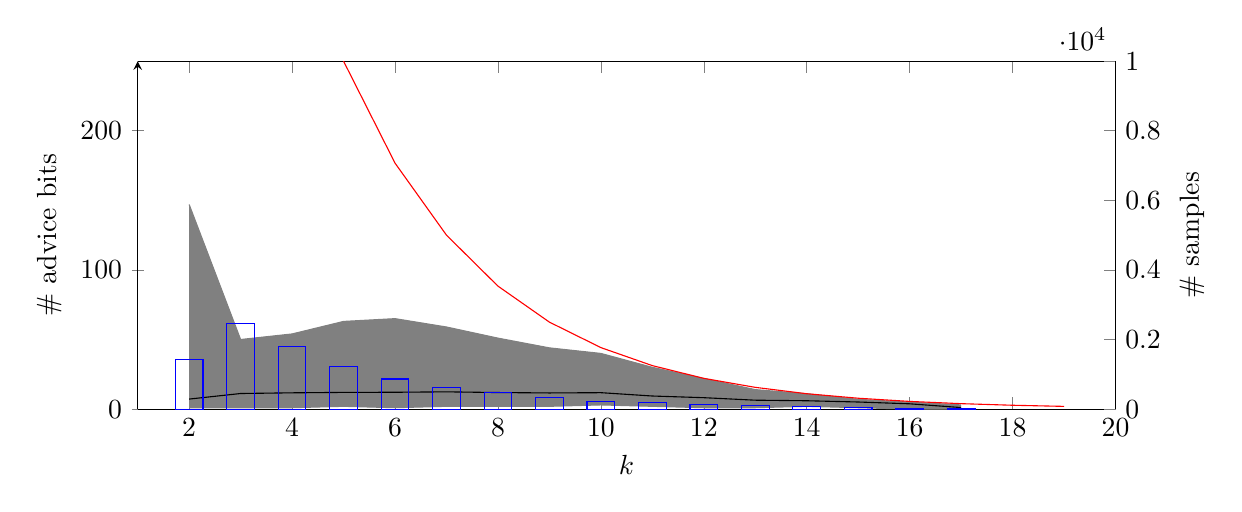
\begin{tikzpicture}
  \begin{axis}[ 
    xlabel=$k$,
    ylabel={\# advice bits},
	legend pos=north west, xmin=1,xmax=20, height=6cm,width=14cm, axis y line=left
  ] 
    \addplot[mark=none,color=gray, stack plots=y] coordinates {
(2,1)
(3,1)
(4,1)
(5,2)
(6,1)
(7,2)
(8,2)
(9,2)
(10,3)
(11,2)
(12,1)
(13,1)
(14,2)
(15,1)
(16,0)
(17,0)




	};

    \addplot[mark=none,fill=gray,draw=none, stack plots=y] coordinates {
(2,146)
(3,49)
(4,53)
(5,61)
(6,64)
(7,57)
(8,49)
(9,42)
(10,37)
(11,28)
(12,21)
(13,13)
(14,9)
(15,6)
(16,5)
(17,3)





	} \closedcycle;

    \addplot[mark=none,color=gray] coordinates {
(2,147)
(3,50)
(4,54)
(5,63)
(6,65)
(7,59)
(8,51)
(9,44)
(10,40)
(11,30)
(12,22)
(13,14)
(14,11)
(15,7)
(16,5)
(17,3)





	};

\addplot[color=black] coordinates {
(2,7.2)
(3,11.2)
(4,11.7)
(5,12)
(6,12.1)
(7,12.4)
(8,11.9)
(9,11.6)
(10,11.8)
(11,9.4)
(12,8.2)
(13,6.4)
(14,6)
(15,5.1)
(16,3.8)
(17,1.1)




};

\addplot[color=red] coordinates {

(5,250)
(6,176.776695296637)
(7,125)
(8,88.3883476483184)
(9,62.5)
(10,44.1941738241592)
(11,31.25)
(12,22.0970869120796)
(13,15.625)
(14,11.0485434560398)
(15,7.8125)
(16,5.5242717280199)
(17,3.90625)
(18,2.76213586400995)
(19,1.953125)



};


  \end{axis}

\begin{axis}[
height=6cm,width=14cm,
      xmin = 1, xmax = 20,
      ymin = 0, ymax = 10000,
      hide x axis,
      axis y line*=right,
      ylabel={\# samples},
      ylabel near ticks, ybar
    ]
      \addplot[blue] coordinates {
(2,1426)
(3,2473)
(4,1803)
(5,1219)
(6,865)
(7,617)
(8,480)
(9,324)
(10,218)
(11,185)
(12,141)
(13,106)
(14,77)
(15,36)
(16,19)
(17,9)





	};
    \end{axis}


\end{tikzpicture}


\end{figure}



\begin{figure}
\caption{{\tt{FF}} gegen {\tt{AA}} für 10000 Instanzen von $G(1000, p)$, III}
\label{fig.exp1.3}
\centering

\subfloat[$p = 0.4$]

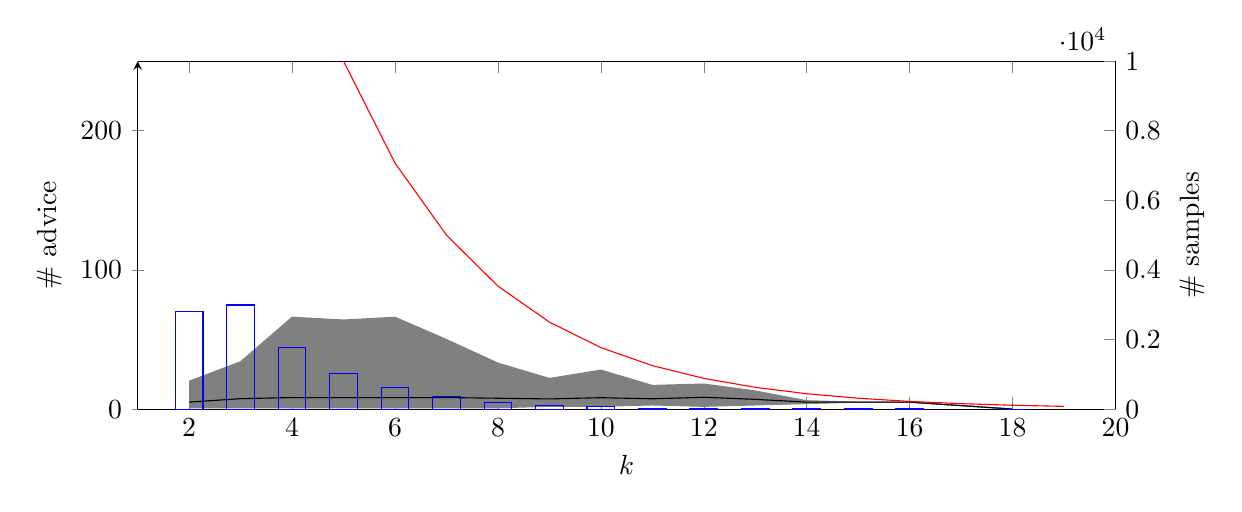
\begin{tikzpicture}
  \begin{axis}[ 
    xlabel=$k$,
    ylabel={\# advice},
	legend pos=north west, xmin=1,xmax=20, height=6cm,width=14cm, axis y line=left
  ] 
    \addplot[mark=none,color=gray, stack plots=y] coordinates {
(2,1)
(3,1)
(4,1)
(5,1)
(6,1)
(7,1)
(8,1)
(9,2)
(10,2)
(11,3)
(12,2)
(13,3)
(14,4)
(15,5)
(16,5)
(18,0)



	};

    \addplot[mark=none,fill=gray,draw=none, stack plots=y] coordinates {
(2,19)
(3,33)
(4,65)
(5,63)
(6,65)
(7,49)
(8,32)
(9,20)
(10,26)
(11,14)
(12,16)
(13,10)
(14,2)
(15,0)
(16,0)
(18,0)




	} \closedcycle;

    \addplot[mark=none,color=gray] coordinates {
(2,20)
(3,34)
(4,66)
(5,64)
(6,66)
(7,50)
(8,33)
(9,22)
(10,28)
(11,17)
(12,18)
(13,13)
(14,6)
(15,5)
(16,5)
(18,0)




	};

\addplot[color=black] coordinates {
(2,5)
(3,7.5)
(4,8.3)
(5,8.2)
(6,8.2)
(7,8.3)
(8,7.8)
(9,7.3)
(10,8.2)
(11,7.4)
(12,8.5)
(13,7)
(14,5)
(15,5)
(16,5)
(18,0)



};

\addplot[color=red] coordinates {

(5,250)
(6,176.776695296637)
(7,125)
(8,88.3883476483184)
(9,62.5)
(10,44.1941738241592)
(11,31.25)
(12,22.0970869120796)
(13,15.625)
(14,11.0485434560398)
(15,7.8125)
(16,5.5242717280199)
(17,3.90625)
(18,2.76213586400995)
(19,1.953125)



};

  \end{axis}
\begin{axis}[
height=6cm,width=14cm,
      xmin = 1, xmax = 20,
      ymin = 0, ymax = 10000,
      hide x axis,
      axis y line*=right,
      ylabel={\# samples},
      ylabel near ticks, ybar
    ]
      \addplot[blue] coordinates {
(2,2796)
(3,2992)
(4,1767)
(5,1023)
(6,630)
(7,351)
(8,198)
(9,99)
(10,72)
(11,29)
(12,26)
(13,9)
(14,3)
(15,2)
(16,2)
(18,1)





	};
    \end{axis}
\end{tikzpicture}

\subfloat[$p = 0.5$]

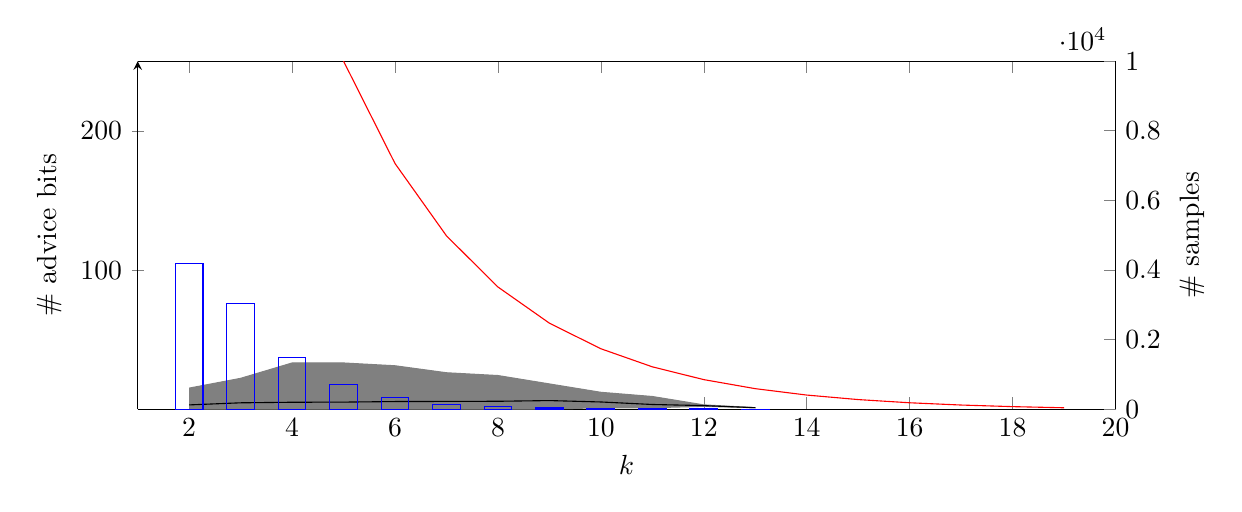
\begin{tikzpicture}
  \begin{axis}[ 
    xlabel=$k$,
    ylabel={\# advice bits},
	legend pos=north west, xmin=1,xmax=20, height=6cm,width=14cm, axis y line=left
  ] 
    \addplot[mark=none,color=gray, stack plots=y] coordinates {
(2,1)
(3,1)
(4,1)
(5,1)
(6,1)
(7,1)
(8,1)
(9,1)
(10,2)
(11,2)
(12,3)
(13,2)




	};

    \addplot[mark=none,fill=gray,draw=none, stack plots=y] coordinates {
(2,15)
(3,22)
(4,33)
(5,33)
(6,31)
(7,26)
(8,24)
(9,18)
(10,11)
(11,8)
(12,1)
(13,0)





	} \closedcycle;

    \addplot[mark=none,color=gray] coordinates {
(2,16)
(3,23)
(4,34)
(5,34)
(6,32)
(7,27)
(8,25)
(9,19)
(10,13)
(11,10)
(12,4)
(13,2)





	};

\addplot[color=black] coordinates {
(2,4)
(3,5.5)
(4,5.9)
(5,6)
(6,6.4)
(7,6.5)
(8,6.6)
(9,7.1)
(10,6.1)
(11,4.3)
(12,3.5)
(13,2)




};

\addplot[color=red] coordinates {

(5,250)
(6,176.776695296637)
(7,125)
(8,88.3883476483184)
(9,62.5)
(10,44.1941738241592)
(11,31.25)
(12,22.0970869120796)
(13,15.625)
(14,11.0485434560398)
(15,7.8125)
(16,5.5242717280199)
(17,3.90625)
(18,2.76213586400995)
(19,1.953125)



};


  \end{axis}

\begin{axis}[
height=6cm,width=14cm,
      xmin = 1, xmax = 20,
      ymin = 0, ymax = 10000,
      hide x axis,
      axis y line*=right,
      ylabel={\# samples},
      ylabel near ticks, ybar
    ]
      \addplot[blue] coordinates {
(2,4190)
(3,3040)
(4,1474)
(5,708)
(6,330)
(7,137)
(8,63)
(9,31)
(10,17)
(11,7)
(12,2)
(13,1)






	};
    \end{axis}

\end{tikzpicture}

\subfloat[$p = 0.6$]

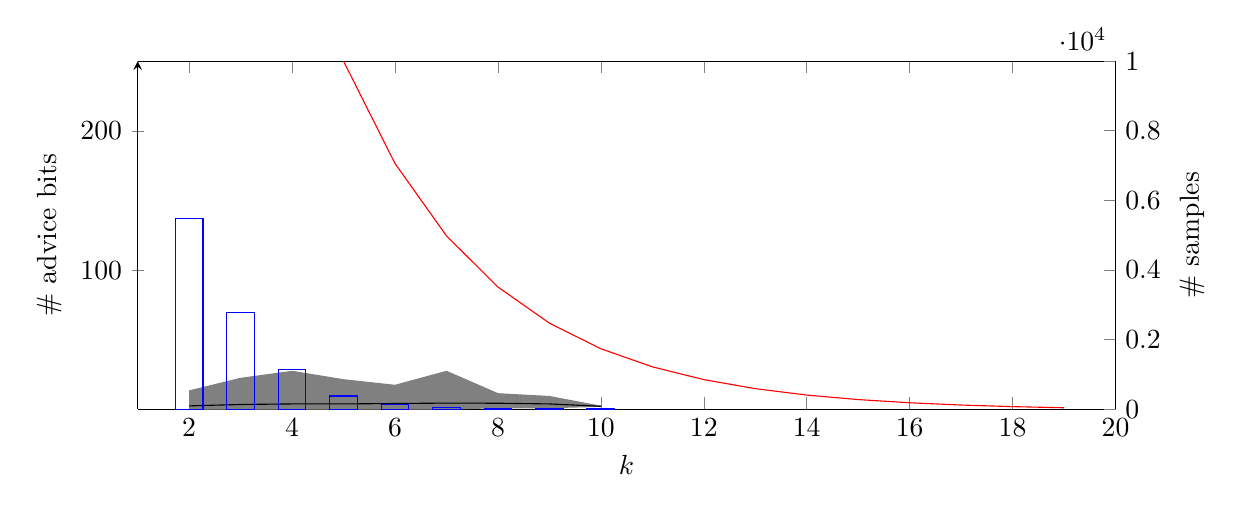
\begin{tikzpicture}
  \begin{axis}[ 
    xlabel=$k$,
    ylabel={\# advice bits},
	legend pos=north west, xmin=1,xmax=20, height=6cm,width=14cm, axis y line=left
  ] 
    \addplot[mark=none,color=gray, stack plots=y] coordinates {
(2,1)
(3,1)
(4,1)
(5,1)
(6,1)
(7,1)
(8,2)
(9,2)
(10,3)





	};

    \addplot[mark=none,fill=gray,draw=none, stack plots=y] coordinates {
(2,13)
(3,22)
(4,27)
(5,21)
(6,17)
(7,27)
(8,10)
(9,8)
(10,0)






	} \closedcycle;

    \addplot[mark=none,color=gray] coordinates {
(2,14)
(3,23)
(4,28)
(5,22)
(6,18)
(7,28)
(8,12)
(9,10)
(10,3)






	};

\addplot[color=black] coordinates {
(2,3.3)
(3,4.3)
(4,4.7)
(5,4.7)
(6,5)
(7,5.3)
(8,5.2)
(9,4.7)
(10,3)





};

\addplot[color=red] coordinates {

(5,250)
(6,176.776695296637)
(7,125)
(8,88.3883476483184)
(9,62.5)
(10,44.1941738241592)
(11,31.25)
(12,22.0970869120796)
(13,15.625)
(14,11.0485434560398)
(15,7.8125)
(16,5.5242717280199)
(17,3.90625)
(18,2.76213586400995)
(19,1.953125)



};


  \end{axis}

\begin{axis}[
height=6cm,width=14cm,
      xmin = 1, xmax = 20,
      ymin = 0, ymax = 10000,
      hide x axis,
      axis y line*=right,
      ylabel={\# samples},
      ylabel near ticks, ybar
    ]
      \addplot[blue] coordinates {
(2,5491)
(3,2788)
(4,1147)
(5,375)
(6,130)
(7,45)
(8,13)
(9,7)
(10,3)







	};
    \end{axis}


\end{tikzpicture}


\end{figure}


Es fallen folgende Dinge auf:

\begin{itemize}
\item Bei sehr kleinen Kantenwahrscheinlichkeiten ($p = 0.01$, $p = 0.02$) ist der First Fit-Algorithmus in der Lage, jeweils immer ungefähr dieselbe Anzahl Farben zu verwenden ($k \in \{6,7,8\}$). Des weiteren kann auch der Algorithmus mit Advice mit dieser Competitive Ratio mithalten, ohne je in die Nähe der Schranke zu kommen.
\item Bei ungefähr $p = 0.05$ ändern sich diese Verhalten jedoch -- die Streuung von $k$ wird breiter für First Fit, und der Algorithmus mit Advice beginnt sich für einzelne Instanzen an die Schranke heranzutasten.
\item Mit stetig grösser werdendem $p$ verschiebt sich die Häufung der $k$s von First Fit nach unten -- dies erscheint logisch, da durch die gestiegene Kantendichte der Informationsgehalt steigt. Ebenso beginnt sich der Bereich der Advice Bits abzuflachen.
\end{itemize}

Der Verlauf von $k$ und der durchschnittlichen Anzahl Advice Bits für den Bereich $p \in (0.01; 0.20 ) $ ist in den Abbildungen~\ref{fig.verlauf} und \ref{fig.verlauf.b} dargestellt. Wir beobachten vor allem, dass ab $p = 0.14$ die Anzahl benötigter Advice Bits wieder zu sinken beginnt, das heisst für $p = 1000$ scheint sich dort die zunehmende Informationsdichte positiv auszuwirken.

\begin{figure}
\caption{$k$  in Abhängigkeit von $p$}
\label{fig.verlauf}
\centering

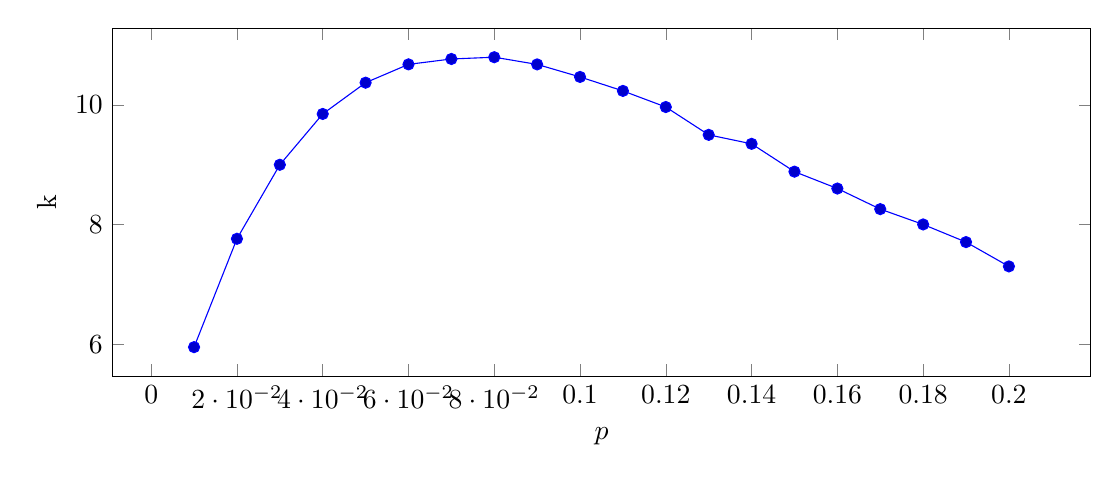
\begin{tikzpicture}
  \begin{axis}[ 
    xlabel=$p$,
    ylabel={k},
	legend pos=north west, height=6cm,width=14cm
  ]

    \addplot coordinates {


(0.01,5.9546)
(0.02,7.7651)
(0.03,9.0022)
(0.04,9.8513)
(0.05,10.3737)
(0.06,10.6799)
(0.07,10.7698)
(0.08,10.7993)
(0.09,10.6793)
(0.1,10.4697)
(0.11,10.2363)
(0.12,9.967)
(0.13,9.502)
(0.14,9.352)
(0.15,8.887)
(0.16,8.605)
(0.17,8.261)
(0.18,8.005)
(0.19,7.71)
(0.2,7.3038)




	};


    \end{axis}


\end{tikzpicture}

\end{figure}


\begin{figure}
\caption{$b$ in Abhängigkeit von $p$}
\label{fig.verlauf.b}
\centering


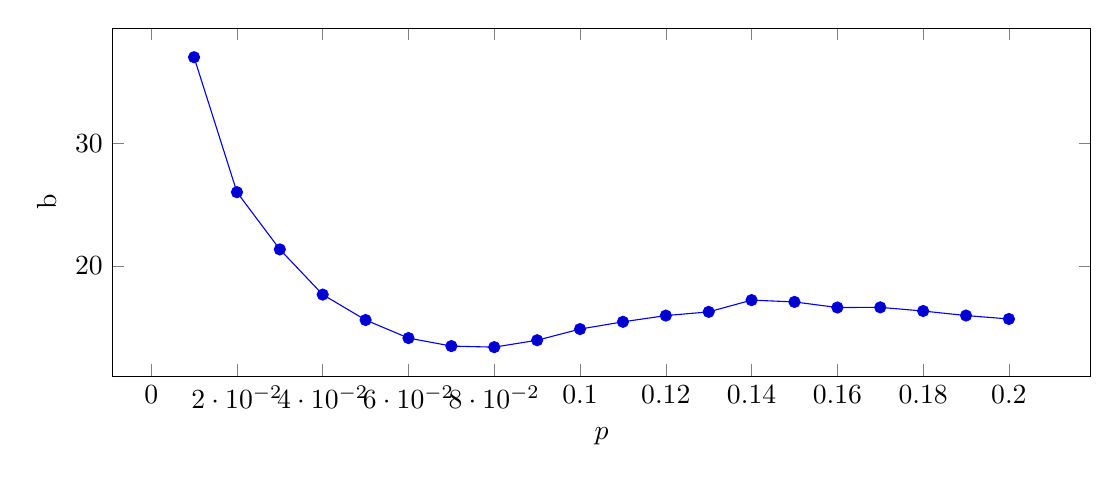
\begin{tikzpicture}
  \begin{axis}[ 
    xlabel=$p$,
    ylabel={b},
	legend pos=north west, height=6cm,width=14cm
  ]



    \addplot coordinates {


(0.01,37.0098)
(0.02,26.0142)
(0.03,21.3515)
(0.04,17.6699)
(0.05,15.599)
(0.06,14.1288)
(0.07,13.4745)
(0.08,13.3896)
(0.09,13.9524)
(0.1,14.8615)
(0.11,15.4523)
(0.12,15.96)
(0.13,16.262)
(0.14,17.221)
(0.15,17.073)
(0.16,16.618)
(0.17,16.63)
(0.18,16.332)
(0.19,15.964)
(0.2,15.6848)



	};

    \end{axis}


\end{tikzpicture}


\end{figure}



\subsection{Anzahl Advice Bits für Optimalität}

In diesem Experiment wollen wir untersuchen, wie viele Advice Bits durchschnittlich benötigt werden, um eine repräsentative Menge von $G(n,p)$-Graphen optimal zu färben. Die Ergebnisse für $n \in (20;990)$ sind je für $p = 0.1$, $p=0.01$ und $p = 0.001$ in den Abbildungen~\ref{fig.verlauf.n01}, \ref{fig.verlauf.n001} und \ref{fig.verlauf.n0001} gegeben.

Dabei fällt auf, dass sich $b$ logarithmisch verhält -- bei $p = 0.01$ ist es offensichtlich, bei den anderen Kantenwahrscheinlichkeiten können wir es zumindest erahnen.

\begin{figure}
\caption{$b$ für $k=2$ in $G(n,0.1)$}
\label{fig.verlauf.n01}
\centering


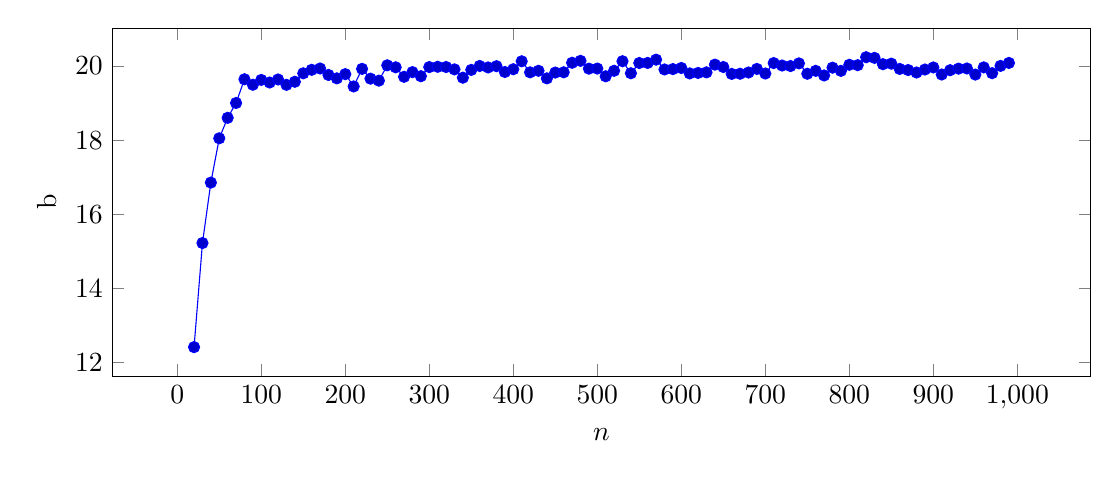
\begin{tikzpicture}
  \begin{axis}[ 
    xlabel=$n$,
    ylabel={b},
	legend pos=north west, height=6cm,width=14cm
  ]



    \addplot coordinates {


(20,12.42)
(30,15.226)
(40,16.8559999999999)
(50,18.05)
(60,18.602)
(70,19.002)
(80,19.642)
(90,19.4939999999999)
(100,19.624)
(110,19.554)
(120,19.636)
(130,19.492)
(140,19.574)
(150,19.8019999999999)
(160,19.8959999999999)
(170,19.9319999999999)
(180,19.758)
(190,19.666)
(200,19.7799999999999)
(210,19.4479999999999)
(220,19.922)
(230,19.6579999999999)
(240,19.6039999999999)
(250,20.0179999999999)
(260,19.964)
(270,19.708)
(280,19.834)
(290,19.724)
(300,19.9699999999999)
(310,19.978)
(320,19.972)
(330,19.9079999999999)
(340,19.684)
(350,19.894)
(360,20)
(370,19.96)
(380,19.994)
(390,19.838)
(400,19.912)
(410,20.126)
(420,19.828)
(430,19.87)
(440,19.666)
(450,19.8219999999999)
(460,19.8299999999999)
(470,20.086)
(480,20.1379999999999)
(490,19.9279999999999)
(500,19.9299999999999)
(510,19.7219999999999)
(520,19.87)
(530,20.128)
(540,19.804)
(550,20.0799999999999)
(560,20.082)
(570,20.17)
(580,19.906)
(590,19.916)
(600,19.9459999999999)
(610,19.7999999999999)
(620,19.8119999999999)
(630,19.828)
(640,20.036)
(650,19.972)
(660,19.7859999999999)
(670,19.7899999999999)
(680,19.824)
(690,19.9199999999999)
(700,19.796)
(710,20.0779999999999)
(720,20.012)
(730,19.9979999999999)
(740,20.0699999999999)
(750,19.79)
(760,19.868)
(770,19.7439999999999)
(780,19.954)
(790,19.8679999999999)
(800,20.0319999999999)
(810,20.022)
(820,20.2359999999999)
(830,20.218)
(840,20.048)
(850,20.0619999999999)
(860,19.9199999999999)
(870,19.8899999999999)
(880,19.824)
(890,19.904)
(900,19.9599999999999)
(910,19.7699999999999)
(920,19.886)
(930,19.9279999999999)
(940,19.932)
(950,19.7679999999999)
(960,19.962)
(970,19.806)
(980,20.002)
(990,20.082)




	};

    \end{axis}


\end{tikzpicture}


\end{figure}


\begin{figure}
\caption{$b$ für $k=2$ in $G(n,0.01)$}
\label{fig.verlauf.n001}
\centering


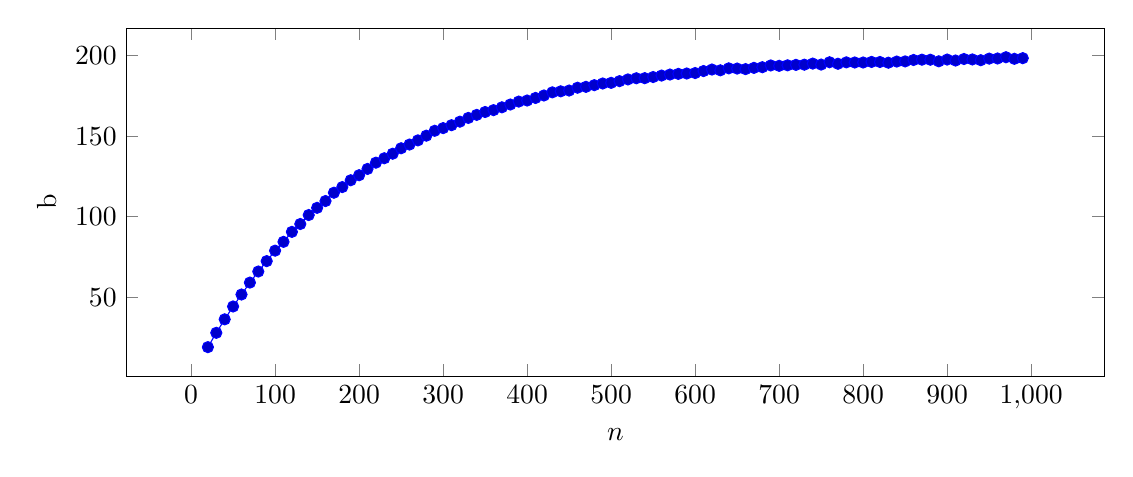
\begin{tikzpicture}
  \begin{axis}[ 
    xlabel=$n$,
    ylabel={b},
	legend pos=north west, height=6cm,width=14cm
  ]



    \addplot coordinates {


(20,19)
(30,27.896)
(40,36.2719999999999)
(50,44.2539999999999)
(60,51.6899999999999)
(70,59.082)
(80,65.9579999999999)
(90,72.412)
(100,78.92)
(110,84.3879999999999)
(120,90.578)
(130,95.464)
(140,101.029999999999)
(150,105.51)
(160,109.723999999999)
(170,114.89)
(180,118.406)
(190,122.638)
(200,125.766)
(210,129.666)
(220,133.563999999999)
(230,136.299999999999)
(240,139.118)
(250,142.509999999999)
(260,144.806)
(270,147.398)
(280,150.309999999999)
(290,153.354)
(300,155.009999999999)
(310,156.83)
(320,159.026)
(330,161.341999999999)
(340,163.228)
(350,165.011999999999)
(360,166.176)
(370,167.931999999999)
(380,169.674)
(390,171.486)
(400,172.15)
(410,173.746)
(420,175.279999999999)
(430,177.219999999999)
(440,177.86)
(450,178.354)
(460,180.093999999999)
(470,180.635999999999)
(480,181.687999999999)
(490,182.728)
(500,183.119999999999)
(510,184.179999999999)
(520,185.253999999999)
(530,185.978)
(540,186.034)
(550,186.734)
(560,187.645999999999)
(570,188.277999999999)
(580,188.692)
(590,188.922)
(600,189.212)
(610,190.446)
(620,191.392)
(630,190.908)
(640,192.133999999999)
(650,191.992)
(660,191.654)
(670,192.417999999999)
(680,192.838)
(690,193.936)
(700,193.688)
(710,194.016)
(720,194.286)
(730,194.396)
(740,195.085999999999)
(750,194.474)
(760,195.917999999999)
(770,194.973999999999)
(780,195.847999999999)
(790,195.765999999999)
(800,195.762)
(810,196.118)
(820,196.078)
(830,195.624)
(840,196.34)
(850,196.444)
(860,197.318)
(870,197.514)
(880,197.48)
(890,196.5)
(900,197.59)
(910,196.983999999999)
(920,197.93)
(930,197.662)
(940,197.186)
(950,198.169999999999)
(960,198.248)
(970,199.04)
(980,198.043999999999)
(990,198.455999999999)





	};

    \end{axis}


\end{tikzpicture}


\end{figure}


\begin{figure}
\caption{$b$ für $k=2$ in $G(n,0.001)$}
\label{fig.verlauf.n0001}
\centering


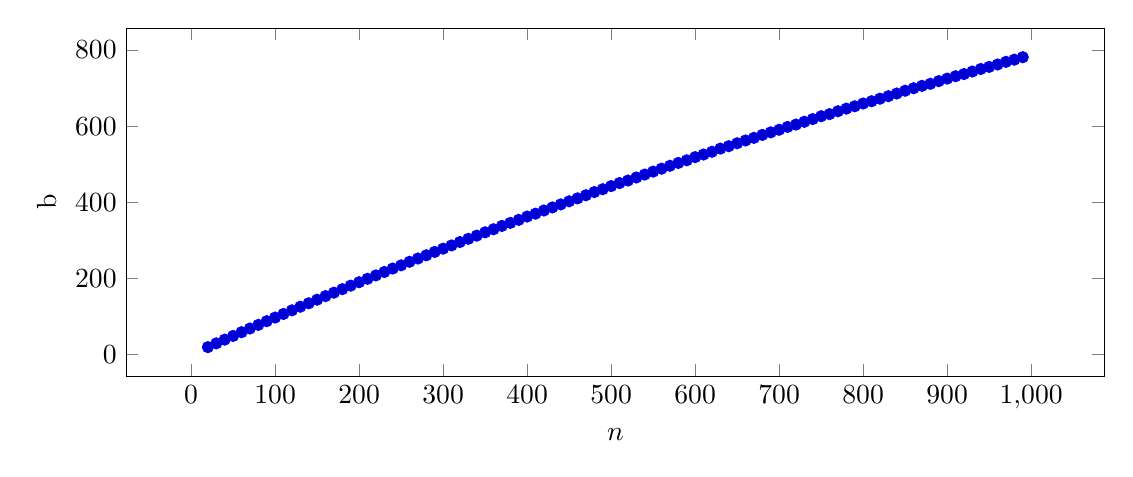
\begin{tikzpicture}
  \begin{axis}[ 
    xlabel=$n$,
    ylabel={b},
	legend pos=north west, height=6cm,width=14cm
  ]



    \addplot coordinates {


(20,19.8999999999999)
(30,29.775)
(40,39.6099999999999)
(50,49.4049999999999)
(60,59.0933333333333)
(70,68.8033333333332)
(80,78.3666666666666)
(90,88.02)
(100,97.6116666666667)
(110,107.018333333333)
(120,116.53)
(130,126.003333333333)
(140,135.063333333333)
(150,144.446666666666)
(160,153.868333333333)
(170,162.911666666666)
(180,172.155)
(190,181.378333333333)
(200,190.388333333333)
(210,199.326666666666)
(220,208.241666666666)
(230,217.244999999999)
(240,226.27)
(250,234.685)
(260,243.983333333333)
(270,252.618333333333)
(280,261.099999999999)
(290,269.953333333333)
(300,278.476666666667)
(310,287.053333333333)
(320,295.883333333333)
(330,304.233333333333)
(340,312.653333333333)
(350,321.364999999999)
(360,329.438333333333)
(370,338.193333333333)
(380,346.136666666666)
(390,354.093333333333)
(400,362.811666666666)
(410,370.333333333333)
(420,378.738333333333)
(430,386.741666666666)
(440,394.709999999999)
(450,402.756666666666)
(460,410.555)
(470,418.701666666666)
(480,427.026666666666)
(490,434.621666666666)
(500,442.745)
(510,450.708333333333)
(520,457.33)
(530,465.276666666666)
(540,473.064999999999)
(550,480.753333333333)
(560,488.448333333333)
(570,496.073333333333)
(580,503.473333333333)
(590,510.501666666666)
(600,518.793333333334)
(610,525.648333333333)
(620,532.818333333333)
(630,541.193333333333)
(640,547.536666666667)
(650,555.188333333333)
(660,562.55)
(670,569.421666666666)
(680,577.174999999999)
(690,583.938333333333)
(700,590.713333333332)
(710,598.059999999999)
(720,604.284999999999)
(730,611.596666666665)
(740,618.731666666667)
(750,626.253333333333)
(760,631.753333333333)
(770,639.285)
(780,646.179999999999)
(790,652.331666666666)
(800,659.598333333334)
(810,665.558333333334)
(820,672.293333333332)
(830,678.873333333333)
(840,685.838333333333)
(850,693.12)
(860,699.681666666666)
(870,705.958333333332)
(880,711.351666666666)
(890,718.326666666666)
(900,724.976666666667)
(910,731.233333333333)
(920,736.925)
(930,743.579999999999)
(940,750.228333333333)
(950,755.756666666666)
(960,762.113333333333)
(970,768.991666666666)
(980,774.748333333333)
(990,781.146666666666)






	};

    \end{axis}


\end{tikzpicture}


\end{figure}


\subsection{Anzahl Advice Bits für $k = 3$}

Zum Abschluss wollen wir noch überprüfen, ob sich für $k = 3$ (und darum für die Competitive Ratio $c = \frac 3 2$) eine Besonderheit ergibt. Dies ist für $p = 0.1$ ebenfalls nicht der Fall, wie in wir auf Abbildung~\ref{fig.verlauf.k3.n01} nachschauen können.

\begin{figure}
\caption{$b$ für $k=3$ in $G(n,0.1)$}
\label{fig.verlauf.k3.n01}
\centering


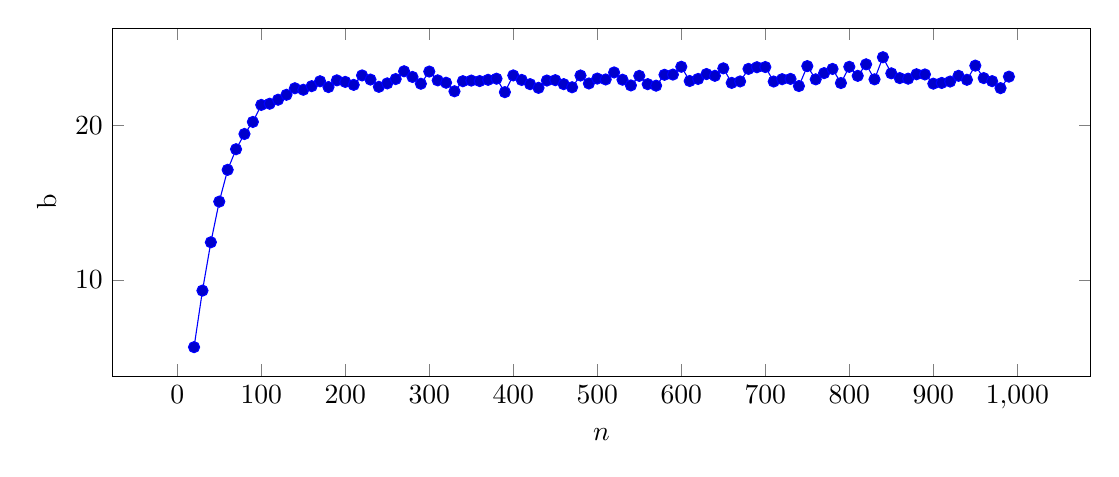
\begin{tikzpicture}
  \begin{axis}[ 
    xlabel=$n$,
    ylabel={b},
	legend pos=north west, height=6cm,width=14cm
  ]



    \addplot coordinates {


(20,5.64199999999999)
(30,9.302)
(40,12.432)
(50,15.0639999999999)
(60,17.1219999999999)
(70,18.458)
(80,19.4439999999999)
(90,20.224)
(100,21.3259999999999)
(110,21.402)
(120,21.662)
(130,21.982)
(140,22.404)
(150,22.306)
(160,22.54)
(170,22.8579999999999)
(180,22.4819999999999)
(190,22.9159999999999)
(200,22.816)
(210,22.624)
(220,23.236)
(230,22.966)
(240,22.496)
(250,22.72)
(260,22.9999999999999)
(270,23.5039999999999)
(280,23.136)
(290,22.696)
(300,23.486)
(310,22.9159999999999)
(320,22.762)
(330,22.208)
(340,22.8619999999999)
(350,22.902)
(360,22.87)
(370,22.95)
(380,23.024)
(390,22.152)
(400,23.236)
(410,22.944)
(420,22.6699999999999)
(430,22.43)
(440,22.904)
(450,22.9279999999999)
(460,22.67)
(470,22.468)
(480,23.23)
(490,22.7139999999999)
(500,23.0319999999999)
(510,22.974)
(520,23.428)
(530,22.9579999999999)
(540,22.588)
(550,23.206)
(560,22.6699999999999)
(570,22.572)
(580,23.276)
(590,23.29)
(600,23.7959999999999)
(610,22.874)
(620,23.008)
(630,23.324)
(640,23.2099999999999)
(650,23.694)
(660,22.752)
(670,22.8459999999999)
(680,23.6579999999999)
(690,23.766)
(700,23.778)
(710,22.84)
(720,22.9919999999999)
(730,23.01)
(740,22.548)
(750,23.838)
(760,22.98)
(770,23.3839999999999)
(780,23.656)
(790,22.7419999999999)
(800,23.792)
(810,23.208)
(820,23.954)
(830,22.982)
(840,24.414)
(850,23.3699999999999)
(860,23.062)
(870,23.0239999999999)
(880,23.3119999999999)
(890,23.2979999999999)
(900,22.702)
(910,22.7479999999999)
(920,22.84)
(930,23.2099999999999)
(940,22.9519999999999)
(950,23.87)
(960,23.0619999999999)
(970,22.864)
(980,22.412)
(990,23.156)





	};

    \end{axis}


\end{tikzpicture}


\end{figure}

\section{Fazit der Experimente}

Es scheint so zu sein, dass die Länge der Probleminstanz $n$ und die Kantendichte $p$ zusammengehören -- sie beide bestimmen am Schluss den Informationsgehalt, den das Online-Problem über die Zeit freigibt. Dieser Informationsgehalt bestimmt in der Konsequenz die quantitative Grenze -- wie wir gesehen haben, nimmt die Steigung von $b$ mit steigender Länge $n$ und konstantem $p$ stetig ab.

\bigskip
Über den Zusammenhang zwischen First Fit und Algorithmus mit Advice lässt sich hingegen folgendes sagen:

\begin{itemize}
\item Für $n = 1000$ scheint die Anzahl benötigter Advices bis $p = 0.14$ zu- und dann wieder leicht abzunehmen. Wir möchten einen Zusammenhang zwischen dieser Bewegungsänderung und $n$ vermuten.
\item Nicht immer kann der Algorithmus mit Advice dasselbe Problem mit exakt derselben Competitive Ratio wie der First Fit Algorithmus lösen: Wenn der Graph (zufällig oder absichtlich) so konstruiert ist, dass es bei zuvielen Knoten, die die Farbe $k-1$ erhalten würden, egal ist, welche Farbe sie bekommen, wird Advice quasi {\sl verschwendet}, was zu einer Verletzung der Schranken führt. Dies ist aber kein Beinbruch --  da der Algorithmus mit Advice dasselbe Problem sogar mit einer besseren Competitive Ratio lösen kann und dabei weniger Advice benötigt.
\end{itemize}


\chapter{Kommentierung der Implementation des Programms {\tt GraphBonanza}}

In den nachfolgenden Abschnitten sollen ein Überblick über die Anforderungen an das Programm sowie deren technische Umsetzung gegeben werden. Wo notwendig, sinnvoll und/oder interessant, werden auch einzelne Code-Abschnitte wiedergegeben und kommentiert.

\section{Anforderungen}

Die primäre Anforderung an das Programm besteht darin, ein Umfeld zu schaffen, worin die Experimente durchgeführt werden können. Ausserdem sollen einzelne Graphen visualisiert werden können.

\section{Umfeld, Architektur und verwendete Bibliotheken}

Das Programm wurde als reine Browser-Lösung unter Verwendung von {\tt HTML} und {\tt JavaScript} umgesetzt. Dadurch ist es theoretisch auf sämtlichen gängigen Plattformen lauffähig und hat keine Abhängigkeiten zu anderen Komponenten und Diensten wie Laufzeitumgebungen, Webservern, Datenbanken oder ähnlichem. Der Nachvollziehbarkeit und der Verwendung durch Dritte ist ebenfalls förderlich, dass kein Compiler vonnöten ist.

In der Praxis wird die Portabilität natürlich eingeschränkt durch die teilweise unvollständige und fehlerhafte Implementierung von {\tt JavaScript}, {\tt HTML} und {\tt CSS} durch veraltete Browser wie zum Beispiel Internet Explorer. Es zeigt sich aber, das das Programm in aktuellen Versionen von {\tt Firefox} und {\tt Chrome} wie erwartet funktioniert.

\bigskip
Das UML-Diagramm in Abbildung~\ref{fig.arch} zeigt einen Überblick über die implementierten Klassen.

Die verwendeten Bibliotheken sind die folgenden:
\begin{itemize}
\item {\tt jQuery} und {\tt jQueryUI} für die Bereitstellung von Controls und Infrastruktur für die Benutzeroberfläche;
\item {\tt knockout.js} für die Vereinfachung des Datenbindings an die Oberfläche;
\item {\tt sigma.js} für die Visualisierung der Graphen.
\end{itemize}

\begin{figure}
\caption{Klassendiagramm von {\tt GraphBonanza}}
\label{fig.arch}
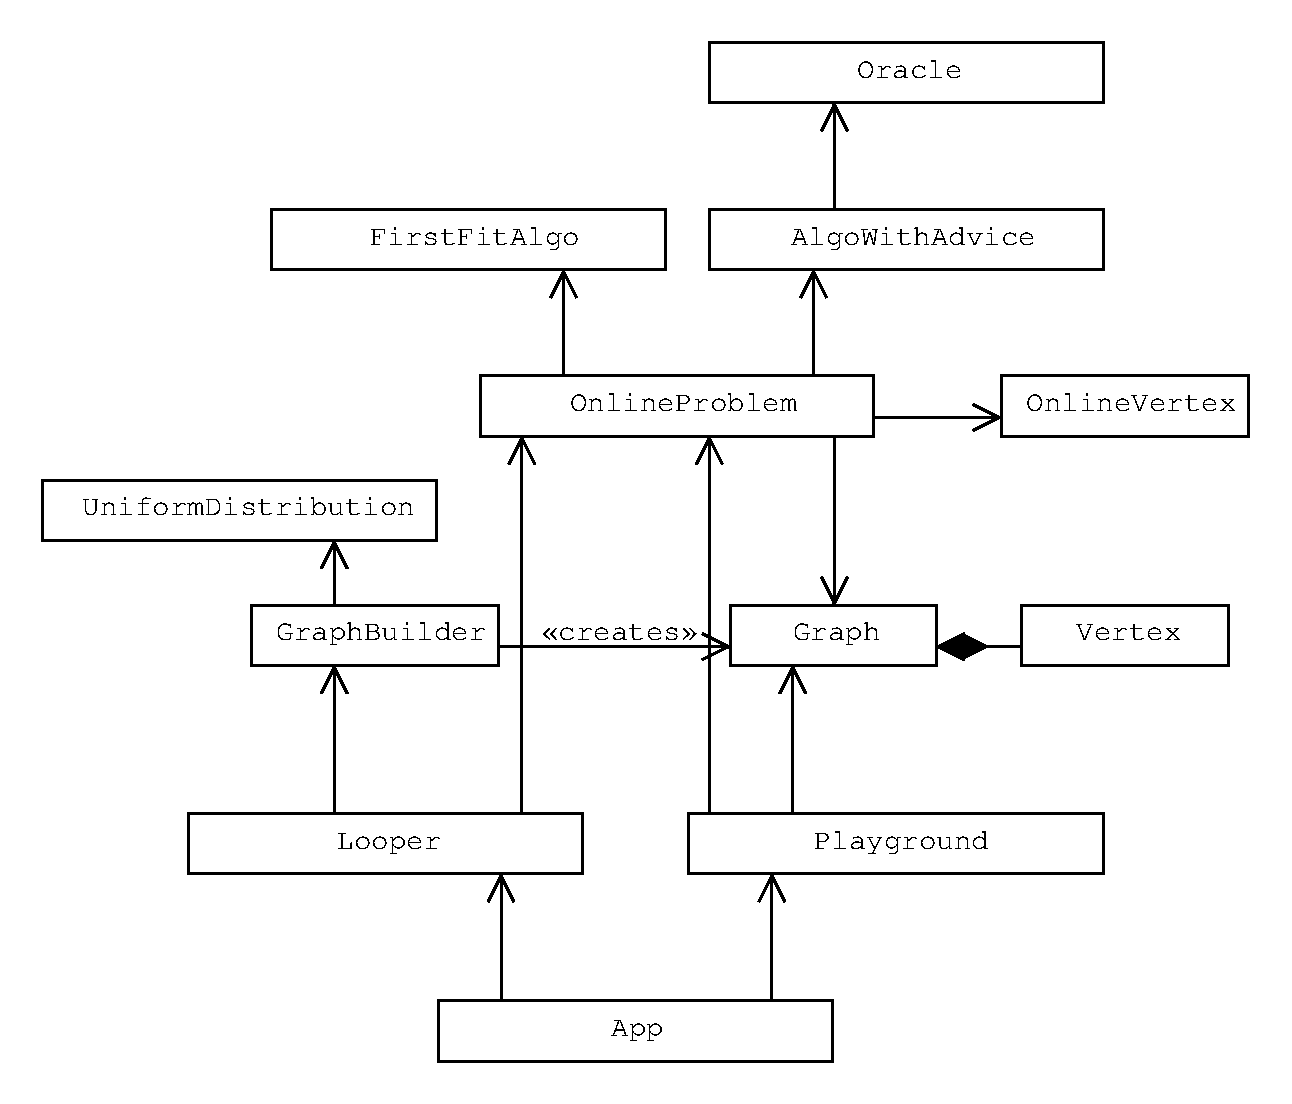
\includegraphics[scale=0.5]{arch.pdf}
\end{figure}

\section{Die {\tt GraphBuilder}-Klasse}

Diese Klasse hat den Zweck, Zufallsgraphen gemäss dem $G(n,p)$-Modell unter Verwendung des optimierten Algorithmus~\ref{gen.opt} herzustellen. Die den optimierten Algorithmus betreffenden Teile der {\tt build()}-Funktion sind in Abbildung~\ref{code.build} abgebildet.

\begin{figure}
\caption{{\tt GraphBuilder::build()}}
\label{code.build}

\begin{lstlisting}
var graph = new Graph();

/* [...] */

var prob = self.probability();
		
var logProb = Math.log(1 - prob);
var e = -1;
while (e < edgeCount) {
	var r = Math.random();
	var k = Math.max(0, Math.ceil(Math.log(r) / logProb - 1));
	e += (k + 1);
			
	var i = e % shore1Count;
	var j = Math.floor(e / shore1Count);
			
	if (i  < shore1.length && j < shore2.length) {
		var v1 = shore1[i];
		var v2 = shore2[j];
		v1.friends.push(v2);
		v2.friends.push(v1);					
	}
}

self.shuffle(graph.verteces);
		
for (var i = 0; i < graph.verteces.length; i++) {
	graph.verteces[i].index = i;
}

return graph;

\end{lstlisting}
\end{figure}

\bibliography{biblio}
\bibliographystyle{plain}

\listoffigures
\listofalgorithms


\end{document}
